\chapter[The Causal Effect of a Merger]{The Causal Effect of a Merger: Bayesian BLP Demand Estimation}\label{ch:blp}

\providecommand{\E}{\mathbb{E}}
\providecommand{\diag}{\mathrm{diag}}
\providecommand{\cH}{\mathcal{H}}
\providecommand{\data}{\mathcal{D}}
\newcommand{\numcorrLa}{0.58}
\newcommand{\numconductacc}{0.98}
\newcommand{\numcovnaive}{0.85}
\newcommand{\numncal}{354}
\newcommand{\numcovavg}{0.94}
\newcommand{\numcovmin}{0.91}
\newcommand{\numpgbcx}{0.98}
\newcommand{\numplogitx}{0.98}
\newcommand{\numpgbcxii}{0.77}
\newcommand{\numplogitxii}{0.47}
\newcommand{\numpgbcxv}{0.08}
\newcommand{\numplogitxv}{0.02}
\newcommand{\numldir}{0.437}
\newcommand{\numldirsd}{0.035}
\newcommand{\numdpdir}{13.0}
\newcommand{\numdpdirsd}{1.5}
\newcommand{\numcsdir}{-0.149}
\newcommand{\numcsdirsd}{0.024}
\newcommand{\numltrue}{0.434}
\newcommand{\numdptrue}{13.3}
\newcommand{\numcstrue}{-0.150}
\newcommand{\numspmicro}{0.047}
\newcommand{\numspnomicro}{0.088}
\newcommand{\numpbert}{1.000}
\newcommand{\numjmracc}{0.16}
\newcommand{\numpharm}{1.00}
\newcommand{\numdplogit}{12.1}
\newcommand{\numinsideshare}{0.60}
\newcommand{\nummeanprice}{3.46}
\newcommand{\numguppia}{1.00}
\newcommand{\numguppib}{1.00}
\newcommand{\numguppic}{1.00}
\newcommand{\numguppid}{1.00}

\newcommand{\nummcnxl}{500}
\newcommand{\nummcboundxl}{4}
\newcommand{\nummcexplxl}{4}
\newcommand{\nummcsprmsegmmxl}{0.111}
\newcommand{\nummcsprmsegbcxl}{0.040}
\newcommand{\nummcspcovgmmxl}{0.95}
\newcommand{\nummcspcovgbcxl}{0.98}
\newcommand{\nummcsprmsenmxl}{0.094}
\newcommand{\nummcspcovnmxl}{0.95}
\newcommand{\nummcsplengbcxl}{0.18}
\newcommand{\nummcsplengmmxl}{0.34}
\newcommand{\nummcsprmseplugxl}{0.111}
\newcommand{\nummcspbiasgmmxl}{-0.022}
\newcommand{\nummcspbiasplugxl}{-0.022}
\newcommand{\nummcsprmsesegmmxl}{0.004}
\newcommand{\nummcsprmsesegbcxl}{0.001}
\newcommand{\nummcdprmsegmmxl}{3.787}
\newcommand{\nummcdprmsegbcxl}{1.131}
\newcommand{\nummcdpcovgmmxl}{0.92}
\newcommand{\nummcdpcovgbcxl}{0.99}
\newcommand{\nummcdprmsenmxl}{1.541}
\newcommand{\nummcdpcovnmxl}{0.97}
\newcommand{\nummcdplengbcxl}{5.64}
\newcommand{\nummcdplengmmxl}{5.84}
\newcommand{\nummcdprmseplugxl}{1.838}
\newcommand{\nummcdpbiasgmmxl}{0.365}
\newcommand{\nummcdpbiasplugxl}{-0.109}
\newcommand{\nummcdprmsesegmmxl}{0.952}
\newcommand{\nummcdprmsesegbcxl}{0.031}
\newcommand{\nummccovsexl}{0.013}
\newcommand{\nummclercovgmmxl}{0.86}
\newcommand{\nummclercovgbcxl}{0.99}
\newcommand{\nummclercovsegmmxl}{0.016}
\newcommand{\nummcfivexln}{500}
\newcommand{\nummcfivexlbound}{279}
\newcommand{\nummcfivesprmsegmmxl}{0.132}
\newcommand{\nummcfivesprmsegbcxl}{0.024}
\newcommand{\nummcfivespcovgmmxl}{0.84}
\newcommand{\nummcfivespcovgbcxl}{1.00}
\newcommand{\nummcfivedprmsegmmxl}{16.898}
\newcommand{\nummcfivedprmsegbcxl}{1.331}
\newcommand{\nummcfivedpcovgmmxl}{0.52}
\newcommand{\nummcfivedpcovgbcxl}{0.98}
\newcommand{\nummcnxv}{500}
\newcommand{\nummcboundxv}{49}
\newcommand{\nummcexplxv}{48}
\newcommand{\nummcsprmsegmmxv}{0.184}
\newcommand{\nummcsprmsegbcxv}{0.059}
\newcommand{\nummcspcovgmmxv}{0.94}
\newcommand{\nummcspcovgbcxv}{0.96}
\newcommand{\nummcsprmsenmxv}{0.097}
\newcommand{\nummcspcovnmxv}{0.98}
\newcommand{\nummcsplengbcxv}{0.25}
\newcommand{\nummcsplengmmxv}{0.49}
\newcommand{\nummcsprmseplugxv}{0.184}
\newcommand{\nummcspbiasgmmxv}{-0.053}
\newcommand{\nummcspbiasplugxv}{-0.053}
\newcommand{\nummcsprmsesegmmxv}{0.006}
\newcommand{\nummcsprmsesegbcxv}{0.002}
\newcommand{\nummcdprmsegmmxv}{96.640}
\newcommand{\nummcdprmsegbcxv}{1.696}
\newcommand{\nummcdpcovgmmxv}{0.88}
\newcommand{\nummcdpcovgbcxv}{0.95}
\newcommand{\nummcdprmsenmxv}{2.012}
\newcommand{\nummcdpcovnmxv}{0.95}
\newcommand{\nummcdplengbcxv}{7.32}
\newcommand{\nummcdplengmmxv}{6.98}
\newcommand{\nummcdprmseplugxv}{2.346}
\newcommand{\nummcdpbiasgmmxv}{9.296}
\newcommand{\nummcdpbiasplugxv}{-0.009}
\newcommand{\nummcdprmsesegmmxv}{46.805}
\newcommand{\nummcdprmsesegbcxv}{0.064}
\newcommand{\nummccovsexv}{0.013}
\newcommand{\nummclercovgmmxv}{0.76}
\newcommand{\nummclercovgbcxv}{1.00}
\newcommand{\nummclercovsegmmxv}{0.019}
\newcommand{\nummcfivexvn}{498}
\newcommand{\nummcfivexvbound}{291}
\newcommand{\nummcfivesprmsegmmxv}{0.147}
\newcommand{\nummcfivesprmsegbcxv}{0.029}
\newcommand{\nummcfivespcovgmmxv}{0.87}
\newcommand{\nummcfivespcovgbcxv}{1.00}
\newcommand{\nummcfivedprmsegmmxv}{22.132}
\newcommand{\nummcfivedprmsegbcxv}{1.158}
\newcommand{\nummcfivedpcovgmmxv}{0.43}
\newcommand{\nummcfivedpcovgbcxv}{1.00}
\newcommand{\nummscollusionalpha}{1.03}
\newcommand{\nummscollusiontrue}{0.0}
\newcommand{\nummscollusiongmm}{9.0}
\newcommand{\nummscollusiongbc}{0.0}
\newcommand{\nummscollusionltrue}{0.572}
\newcommand{\nummscollusionlgmm}{0.347}
\newcommand{\nummscollusionlgbc}{0.605}
\newcommand{\nummscollusionpc}{1.000}
\newcommand{\nummsperfectalpha}{0.97}
\newcommand{\nummsperfecttrue}{0.0}
\newcommand{\nummsperfectgmm}{38.4}
\newcommand{\nummsperfectgbc}{0.0}
\newcommand{\nummsperfectltrue}{0.000}
\newcommand{\nummsperfectlgmm}{0.900}
\newcommand{\nummsperfectlgbc}{0.000}
\newcommand{\nummsperfectpc}{1.000}
\newcommand{\nummspartgmmbiasdp}{3.25}
\newcommand{\nummspartgmmrmsedp}{3.74}
\newcommand{\nummspartgmmbiasler}{-0.126}
\newcommand{\nummspartgmmrmseler}{0.129}
\newcommand{\nummspartgmmsedp}{0.19}
\newcommand{\nummspartgbcbiasdp}{2.99}
\newcommand{\nummspartgbcrmsedp}{3.58}
\newcommand{\nummspartgbcbiasler}{-0.108}
\newcommand{\nummspartgbcrmseler}{0.118}
\newcommand{\nummspartgbcsedp}{0.20}
\newcommand{\nummsparttruedp}{7.10}
\newcommand{\nummsparttruebertdp}{10.81}
\newcommand{\nummsparttrueler}{0.507}
\newcommand{\nummspartn}{100}
\newcommand{\nummspartpcbert}{0.93}
\newcommand{\nummspartpccoll}{0.07}
\newcommand{\nummspartpcperf}{0.00}

\newcommand{\numcerdpmtrue}{8.6}
\newcommand{\numcerdprtrue}{3.2}
\newcommand{\numcerdpmgbc}{9.0}
\newcommand{\numcerdpmgbcsd}{1.4}
\newcommand{\numcerdprgbc}{3.0}
\newcommand{\numcerdprgbcsd}{1.3}
\newcommand{\numcerdpmgmm}{7.1}
\newcommand{\numcerdprgmm}{2.7}
\newcommand{\numcerdpmgmmsd}{1.0}
\newcommand{\numcerdprgmmsd}{0.4}
\newcommand{\numcerdpmlogit}{6.7}
\newcommand{\numcerdprlogit}{2.6}
\newcommand{\numcerpmgbc}{1.00}
\newcommand{\numcerprgbc}{0.01}
\newcommand{\numcerpmgmm}{1.00}
\newcommand{\numcerprgmm}{0.00}
\newcommand{\numcercsmtrue}{-0.079}
\newcommand{\numcercsrtrue}{-0.044}
\newcommand{\numcercsmgbc}{-0.081}
\newcommand{\numcercsrgbc}{-0.042}
\newcommand{\numcerltrue}{0.431}
\newcommand{\numcerlgbc}{0.422}
\newcommand{\numcershA}{19.6}
\newcommand{\numcershB}{12.3}
\newcommand{\numcershC}{15.4}
\newcommand{\numcershD}{8.7}
\newcommand{\numcerinside}{56.1}
\newcommand{\numcerprgbcnabove}{10}
\newcommand{\numcerngbcdraws}{1{,}500}
\newcommand{\numcerdprgbcqlo}{1.95}
\newcommand{\numcerdprgbcqhi}{4.14}
\newcommand{\numcerdprgmmqlo}{2.43}
\newcommand{\numcerdprgmmqhi}{3.55}


\begin{tcolorbox}[colback=gray!6,colframe=gray!50,title=In brief,fonttitle=\normalfont\itshape,coltitle=black,colbacktitle=gray!15,boxrule=0.4pt,arc=1pt]
A merger is the intervention $\mathrm{do}(H := H^{\mathrm{post}})$ on the form of competition, with no treated unit, so its price effect can only come from a model. Under modularity and given the premerger data, it depends on the three nonlinear demand parameters and the form of competition alone, and the agency's answer is a pushforward posterior. Markups are the hinge: the Lerner index, upward pricing pressure and the merger price effect follow from the markup map, and diversion from the demand parameters. Orthogonal moments fall short here, because the target is a nonlinear fixed point, the moments are flat at zero heterogeneity, conduct is a discrete parameter and the decision needs a probability. Generative Bayesian computation simulates industries and learns the posterior of the estimands and of conduct from summary statistics. With 15 markets, over \nummcnxv{} simulated industries at one true parameter value and on the same aggregate data, its root mean squared error for the merger price effect is \nummcdprmsenmxv{} percentage points against \nummcdprmseplugxv{} for the usual BLP moment estimator at its point estimate, whose Krinsky and Robb draws explode in \nummcexplxv{} of those industries. In one simulated collusive industry that estimator predicts a \nummscollusiongmm\% price rise where the truth is \nummscollusiontrue\%, while the posterior puts probability \nummscollusionpc{} on collusion. The applications are a minivan merger and a cereal merger with a divestiture remedy.
\end{tcolorbox}

A merger\index{merger|textbf} is a treatment applied once, to one industry, and never at random. The competition authority must predict its effect on prices before it happens, when the merged industry does not yet exist. If the fundamental problem of causal inference is that we never see both potential outcomes for the same unit, merger review is its limiting case: we see neither the treated outcome nor any treated unit.

The only route to the answer is a model of how the treatment works. A merger changes who sets which prices, and prices move because firms reoptimize in a new equilibrium. The causal effect is a function of model parameters and its posterior is the object of inference. The question is how to compute that posterior when the model is an equilibrium of a random coefficients demand system.

The workhorse model is the random coefficients logit\index{random coefficients logit|textbf} of Berry, Levinsohn and Pakes (1995)\index{Berry Levinsohn Pakes model|see{BLP demand model}}, known as BLP\index{BLP demand model|textbf}\index{BLP|see{BLP demand model}}. It is estimated by the generalized method of moments (GMM), and its estimates feed the merger simulations\index{merger simulation|textbf}, diversion ratios and upward pricing pressure\index{upward pricing pressure} screens of agencies and courts (Nevo 2000; Farrell and Shapiro 2010; Miller and Weinberg 2017). We develop a Bayesian alternative organized around one fact: every antitrust\index{antitrust|textbf} quantity is a function of the markup vector and the demand parameters, and the markup vector, given the data, depends on only two unknowns: the nonlinear demand parameters $\theta_2$ and the form of competition $H$.

We use generative Bayesian computation\index{generative Bayesian computation} (GBC) to learn the posterior.

\section{The merger as an intervention}\label{blp:sec:causal}

We define potential prices\index{potential prices|textbf} under each form of competition and state modularity, the assumption that carries the premerger estimates to the merger counterfactual. Modularity is not enough: the nonlinear demand parameters and conduct must themselves be identified, through the instruments and the separation results of the chapter. The payoff is Proposition~\ref{blp:prop:ident}: given the data, the price effect of a merger depends only on three nonlinear demand parameters and a discrete conduct parameter, so the agency's question is a question about the posterior of $(\theta_2,H)$.

\subsection{Potential prices and the structural causal model}

Index markets by $t=1,\dots,T$ and products by $j=1,\dots,J$. An ownership structure, or more
generally a conduct, is a matrix $H$ in a finite set $\cH$ (Section~\ref{blp:sec:model}), except that perfect competition enters as a label $H^P$ for zero markups. For each $h\in\cH$ write $\bm p_t(h)$ and $\bm s_t(h)$ for the prices
and shares that market $t$ would exhibit if conduct were $h$. These are potential outcomes\index{potential outcomes} in the
sense of Rubin (1974). We observe $\bm p_t = \bm p_t(H)$ for the prevailing $H$; a merger that changes conduct to $H^{\mathrm{post}}$ has causal effect
\[
\Delta\bm p_t \;=\; \bm p_t(H^{\mathrm{post}}) - \bm p_t(H).
\]
No market has ever been observed under $H^{\mathrm{post}}$.

Potential prices\index{potential prices} are generated by a structural causal model\index{structural causal model}\index{structural causal model!of the merger|textbf} in the sense of Pearl (2009). Exogenous variables are product characteristics $\bm x_t$, cost shifters\index{cost shifter|textbf} $\bm w_t$, unobserved
demand shocks\index{demand shock|textbf} $\bm\xi_t$ (quality the econometrician does not see) and cost shocks $\bm\omega_t$.
The structural equations are
\begin{equation}\label{blp:eq:scm}
\delta_t = \bm x_t^\top\beta + \bm\xi_t,\qquad
\bm c_t = \bm w_t^\top\gamma + \bm\omega_t,\qquad
(\bm p_t,\bm s_t) = \mathrm{Eq}(\delta_t,\bm x_{1t},\bm c_t;\theta_2,H),
\end{equation}
where $\mathrm{Eq}$ returns the equilibrium of the pricing game with demand $\theta_2$, mean
utilities $\delta_t$, the characteristic $\bm x_{1t}$ that carries the random coefficient, marginal costs\index{marginal cost|textbf} $\bm c_t$ and conduct $H$; we assume this equilibrium is unique, or that $\mathrm{Eq}$ applies a fixed selection rule. A merger is the intervention\index{merger!as an intervention|textbf}
$\mathrm{do}(H := H^{\mathrm{post}})$\index{do operator}. Figure~\ref{blp:fig:dag} draws the graph.

\begin{figure}[htbp]
\centering
\begin{tikzpicture}[
  node distance=1.1cm and 1.5cm,
  v/.style={circle, draw=#1, fill=#1!12, very thick, minimum size=0.95cm, font=\small},
  u/.style={circle, draw=#1, fill=#1!12, very thick, dashed, minimum size=0.95cm, font=\small},
  arr/.style={-{Stealth[length=2.4mm]}, very thick, draw=black!60}]
\node[v=gbc] (x) {$\bm x$};
\node[u=jmr, below=of x] (xi) {$\bm\xi$};
\node[v=aqua, below=of xi] (w) {$\bm w$};
\node[u=jmr, below=of w] (om) {$\bm\omega$};
\node[v=gbc, right=2.2cm of x] (d) {$\delta$};
\node[v=aqua, right=2.2cm of w] (c) {$\bm c$};
\node[v=sand, right=2.0cm of $(d)!0.5!(c)$] (p) {$\bm p$};
\node[v=gbc, right=1.6cm of p] (s) {$\bm s$};
\node[v=jmr, above=2.9cm of p] (H) {$H$};
\node[font=\footnotesize, text=black!60, right=0.1cm of H] {$\mathrm{do}(H := H^{\mathrm{post}})$};
\draw[arr] (x) -- (d); \draw[arr] (xi) -- (d); \draw[arr] (w) -- (c); \draw[arr] (om) -- (c);
\draw[arr] (d) -- (p); \draw[arr] (c) -- (p); \draw[arr] (H) -- (p); \draw[arr] (p) -- (s);
\draw[arr] (d) to[bend left=22] (s);
\end{tikzpicture}
\caption{The structural causal model of a differentiated products market. Dashed nodes are
unobserved. The demand shock $\bm\xi$ moves both prices (through the equilibrium) and shares, so
it confounds the effect of price on demand; the cost shifter $\bm w$ moves prices only through
costs and is an instrument. A merger is the intervention $\mathrm{do}(H := H^{\mathrm{post}})$. The graph omits four paths of the model: the correlation between $\bm\xi$ and $\bm\omega$ and the dependence of cost on the characteristic $x_1$, both of which the simulations use (Section~\ref{blp:sec:model}), and the direct effects of $x_1$ on prices and shares through its random coefficient.}
\label{blp:fig:dag}
\end{figure}

\begin{assumption}[Modularity]\label{blp:ass:mod}
The intervention $\mathrm{do}(H := H^{\mathrm{post}})$ replaces $H$ in the equilibrium equation of
\eqref{blp:eq:scm} and leaves the other structural equations, the parameters $(\beta,\gamma,\theta_2)$
and the exogenous variables unchanged.
\end{assumption}

Modularity\index{modularity|textbf} is the substantive content of a merger simulation: product qualities and costs are unchanged. It rules out merger efficiencies\index{merger!efficiencies|textbf} and repositioning, which can be added as explicit changes to $\bm c_t$ or $\delta_t$ when evidence supports them.



\subsection{Three features of this causal problem}

\medskip\noindent\textit{The estimand is a model parameter.}\enspace With no population of merged industries, a model free average of potential outcomes is unavailable even in principle. The effect $\Delta\bm p_t$ is defined only through the
structural model, product by product and market by market. This is the model first view of Chapter~\ref{ch:mccullagh}: treat the effect as determined by the model's parameters, not as an average over observed units. Merger review leaves no alternative.

\medskip\noindent\textit{Interference is the mechanism.}\index{interference}\index{interference!in markets|textbf}\enspace The stable unit treatment value
assumption\index{stable unit treatment value assumption} fails by design. When firms A and B merge, the price of a rival's product (C1 in the application of Section~\ref{blp:sec:app}) changes although its ownership does not, because the rival best responds to higher prices of its substitutes: the outcome of product $k$ depends on the treatment of products $j\neq k$. The equilibrium in \eqref{blp:eq:scm} fully specifies this interference, and Proposition~\ref{blp:prop:firstorder} gives its first order form.

\medskip\noindent\textit{Price is confounded.}\index{confounding!price endogeneity|textbf}\enspace The demand curve $p\mapsto s_j(p)$ is a dose response function whose slope is the causal effect of price on demand. Firms set higher prices for products with high unobserved quality $\xi_{jt}$, so
$\xi$ confounds the regression of shares on prices\index{price endogeneity|textbf}. In the graph of Figure~\ref{blp:fig:dag} the part of the cost shifter $\bm w_t$ excluded from utility is an instrument\index{instrumental variable}: it moves prices through costs (relevance), is independent of $\bm\xi_t$ (exogeneity), and affects shares only through prices (exclusion). Rivals' characteristics also qualify, since they shift a product's markup without entering its utility. 

\paragraph{Retrospective evaluation.}\index{merger retrospective|textbf} Once a merger is allowed, a difference in differences\index{difference in differences}\index{difference in differences!in the merger setting|textbf} design can compare price changes in affected and control markets (Chapter~\ref{ch:did}). Ashenfelter and Hosken (2010) study five consumer product mergers this way; Weinberg (2008) surveys earlier work. These retrospectives, antitrust's closest thing to an experiment, serve as posterior predictive checks\index{posterior predictive check}: treat the estimate as a noisy observation of the merging parties' realized price effect and compute the posterior predictive probability of a value at least as extreme (Exercise~\ref{blp:ex:retro}). Repeated small probabilities indicate misspecification in demand, conduct or modularity. Retrospectives cannot replace the structural model, because they arrive after the decision and describe cleared mergers rather than the one under review, but the prior for conduct and efficiencies in the next case should be built on them.

\section[Orthogonal moments and BLP GMM]{Orthogonal moments, BLP GMM and what a posterior adds}\label{blp:sec:dml}

BLP GMM\index{BLP GMM|textbf}\index{GMM|see{BLP GMM}} is a semiparametric moment estimator of the kind discussed in Chapters~\ref{ch:dml} to~\ref{ch:critique}. For fixed $\theta_2$ the linear parameters $\beta$ are concentrated out by
instrumental variables, and $\theta_2$ is chosen to set the instrument moments
$T^{-1}\sum_t Z_t^\top\bm\xi_t(\theta_2)$ close to zero. Because $\beta$ is profiled, the
concentrated criterion is insensitive to first order to errors in $\beta$, an orthogonality
property\index{Neyman orthogonality} in the sense of Chernozhukov and coauthors (2018). The nuisance parameters $(\beta,\gamma)$ and
the distribution of $(\bm\xi,\bm\omega)$ are left unmodelled. In the notation of Chapter~\ref{ch:dml}, with $W_t = (\bm s_t,\bm p_t,\bm x_t,Z_t)$ the data of market $t$, the target is $\theta_2$, the nuisance that enters the moments is $\beta$, and the score is $\psi(W_t;\theta_2,\beta) = Z_t^\top\{\delta_t(\theta_2)-\bm x_t^\top\beta\}$. The displayed score becomes orthogonal in $\beta$ once the instruments are replaced by the linear combinations of them that are uncorrelated with $\bm x_t$, and Exercise~\ref{blp:ex:dml} asks the reader to check the orthogonality claim in that form.

Orthogonality buys an approximately normal $\hat\theta_2$ when $T$ is large and $\theta_2$ is
interior. It does not deliver the causal estimand, for four of the reasons that Section~\ref{blp:sec:why} sets out: the target is a nonlinear functional defined by a fixed point, the moments are flat near zero heterogeneity, conduct is a discrete nuisance that changes the target, and the decision needs a probability.

\section[Why Bayes for antitrust]{Bayesian methods and BLP GMM in antitrust}\label{blp:sec:why}

BLP GMM is consistent and, with optimal instruments, efficient as the number of markets grows, if the model is correctly specified. Merger review\index{antitrust} is different: a decision about a few nonlinear functionals, made from whatever markets the data cover, which may be few, with the
form of competition in doubt. A Bayesian treatment is better suited on seven counts; the propositions cited below are stated later in the chapter.

\medskip\noindent\textit{1. The estimands are nonlinear.}\enspace The merger price effect
$e = g(\theta_2,H)$ is defined by a fixed point (Proposition~\ref{blp:prop:merger}) and is convex in
price sensitivity under logit demand, since markups then scale like $1/\alpha$. GMM reports $g(\hat\theta_2)$ with a delta
method\index{delta method} or Krinsky and Robb\index{Krinsky and Robb draws|textbf} (1986) interval built on a normal approximation to
$\hat\theta_2$, and, on top of any finite sample bias of $\hat\theta_2$, carries the curvature bias $\tfrac12\mathrm{tr}\{\nabla^2 g\,\mathcal V\}$ of
Proposition~\ref{blp:prop:pushforward}. A Krinsky and Robb interval draws $\theta_2$ from that normal approximation and pushes each draw through the equilibrium; in the Monte Carlo below, the GMM point estimate of a derived quantity is the median of those draws, with the plug in $g(\hat\theta_2)$ reported beside it. GBC learns the pushforward posterior of $e$ directly and linearizes nothing.

\medskip\noindent\textit{2. Variance parameters sit near a boundary.}\index{boundary parameter|textbf}\enspace Random coefficient scales are nonnegative and often small. Near zero the GMM estimator has a point mass
at the boundary and Wald intervals are invalid (Andrews 1999); with many products the
nonlinear parameters can be weakly identified (Armstrong 2016). Proposition~\ref{blp:prop:flat}
shows why: at zero the shares do not move to first order in $\sigma$, so the moments identify only
$\sigma^2$. A posterior on $[0,\infty)$ needs no special treatment. 

\medskip\noindent\textit{3. Conduct is uncertain.}\index{conduct|textbf}\enspace BLP GMM\index{BLP GMM} and the equilibrium likelihood of Viard, Gron and Polson (2015, VGP below) maintain
Bertrand Nash. A merger of two colluding firms\index{collusion} changes nothing under joint monopoly but is the main event under Bertrand Nash. A Bayesian treats $H$ as a parameter, reports $\Prob(H\mid\data)$ and
averages the merger prediction over conduct models (Proposition~\ref{blp:prop:bma}). 

\medskip\noindent\textit{4. Micro data enter through their sampling distribution.}\enspace
Petrin (2002) showed that moments linking demographics to vehicle choice pin down heterogeneity in price sensitivity. GMM must stack and weight micro and aggregate moments, and the
answer depends on the weights. GBC simulates the micro moments with their survey noise and the network learns how informative they are.

\medskip\noindent\textit{5. Decisions need probabilities.}\enspace An agency decides whether to challenge, and the relevant input is $\Prob(\Delta p/p > r\mid\data)$ for a threshold such as the 5\%
price rise, weighed against the costs of the two errors (Proposition~\ref{blp:prop:decision}). A posterior delivers this probability; a confidence interval does not.

\medskip\noindent\textit{6. Samples can be small.}\enspace With few markets the asymptotic approximation behind GMM standard errors has little to work with, as the 15 market simulations of Section~\ref{blp:sec:mc} show; the GMM objective is
nonconvex and sensitive to starting values and the contraction tolerance
(Dub\'e, Fox and Su 2012; Knittel and Metaxoglou 2014). GBC never optimizes that objective.

\medskip\noindent\textit{7. Calibration can be checked in advance.}\enspace The GBC posterior is a
trained map, so its coverage can be measured on hundreds of simulated industries at the observed
design before use; the same check for GMM or MCMC requires hundreds of refits.

\medskip\noindent\textit{When GMM is enough.}\enspace With many markets, strong instruments,
parameters away from the boundary, known conduct and nearly linear estimands, the quasi posterior of the GMM criterion and
the sampling distribution of efficient GMM agree to first order by a Bernstein von Mises argument\index{Bernstein von Mises theorem}
(Chernozhukov and Hong 2003). GBC does not cure misspecified demand, and its
efficiency is bounded by its summaries (Table~\ref{blp:tab:compare}). The case for Bayes is strongest
where markets are few, conduct is in doubt and the decision needs a probability.

\section{The model}\label{blp:sec:model}\index{structural estimation}

The demand half is the random coefficients logit\index{random coefficients logit}\index{BLP demand model}, whose nonlinear parameters $\theta_2$ govern substitution and so how much a merged firm gains by raising a price. The supply half is a pricing game indexed by a conduct matrix $H$, which says whose profits each price is set to maximize; a merger is a change in $H$.

\subsection{Demand}
There are $T$ markets with $J$ products each. Consumer $i$ in market $t$ has utility\index{mean utility|textbf}
\begin{equation}\label{blp:eq:utility}
  u_{ijt} = \underbrace{\bm x_{jt}^\top \beta + \xi_{jt}}_{\delta_{jt}}
  \;-\; \alpha_i\, p_{jt} \;+\; \sigma_x \eta_i\, x_{1jt} \;+\; \varepsilon_{ijt},
  \qquad \alpha_i = \alpha\, e^{-\sigma_p \nu_i},
\end{equation}
for $j=1,\dots,J$, and $u_{i0t} = \varepsilon_{i0t}$ for the outside good\index{outside good|textbf}, with
$\varepsilon_{ijt}$ independent type I extreme value. As in Petrin (2002) and Nevo (2001),
$\nu_i$ is an observed demographic (standardized log income, distributed $N(0,1)$) and
$\eta_i\sim N(0,1)$ is an unobserved taste for $x_1$. The price coefficient is lognormal, so
$\alpha_i>0$ for every consumer and $\E[\alpha_i] = \alpha e^{\sigma_p^2/2}$. The nonlinear
parameters are $\theta_2 = (\alpha,\sigma_p,\sigma_x)\in\Theta_2 = (0,\infty)\times[0,\infty)^2$.
Individual choice probabilities and shares are
\begin{gather}\label{blp:eq:shares}
  s_{ijt} = \frac{\exp(V_{ijt})}{1 + \sum_k \exp(V_{ikt})},\qquad
  s_{jt} = \int s_{ijt}\, dF(\nu_i,\eta_i),\\
  V_{ijt} = \delta_{jt} - \alpha_i p_{jt} + \sigma_x\eta_i x_{1jt}.\notag
\end{gather}
For each $\theta_2$ and $\bm p_t$, the map $\delta_t\mapsto\bm s_t$ is a bijection from
$\mathbb R^J$ onto the open simplex (Berry 1994)\index{share inversion|textbf}, and the contraction\index{BLP contraction|textbf}
$\delta \leftarrow \delta + \log \bm s^{\mathrm{obs}} - \log \bm s(\delta)$ computes its inverse
$\delta_t(\theta_2)$ (Berry, Levinsohn and Pakes 1995).

\subsection{Supply and the form of competition}
Marginal cost\index{marginal cost} is $c_{jt} = \bm w_{jt}^\top\gamma + \omega_{jt}$, where $\bm w_{jt}$ contains a
cost shifter excluded from demand. A conduct model\index{conduct} is a matrix $H\in\cH = \{H^{B}, H^{M}, H^{P}\}$
with $H_{jk}=1$ when the price of $j$ is set taking account of the profit on $k$, and $H_{jj}=1$:
\begin{itemize}
\item Bertrand Nash\index{Bertrand Nash equilibrium|textbf}, $H^B$: $H_{jk} = 1$ if and only if $j$ and $k$ have the same owner;
\item joint monopoly\index{joint monopoly|textbf}, $H^M$: $H_{jk}=1$ for all $j,k$;
\item perfect competition, $H^P$: prices equal marginal costs, so $\bm m = 0$. Here $H^P$ labels the case $\bm m = 0$ and is not an ownership matrix, because every $0/1$ matrix with unit diagonal gives strictly positive markups by the argument of Lemma~\ref{blp:lem:dd}.
\end{itemize}
Let $D_p$ have entries $(D_p)_{jk} = \partial s_j/\partial p_k$. For $H\in\{H^B,H^M\}$ the first
order conditions\index{first order condition of the pricing game|textbf} are $\bm s + (H\odot D_p^\top)\bm m = 0$ with $\bm m = \bm p - \bm c$. Under
\eqref{blp:eq:utility},
\begin{equation}\label{blp:eq:jacobian}
  \frac{\partial s_j}{\partial p_k} = -\int \alpha_i s_{ij}\bigl(\mathbf 1\{j=k\} - s_{ik}\bigr)dF
  \;=\; -\Lambda_{jj}\mathbf 1\{j=k\} + \Gamma_{jk},
\end{equation}
where $\Lambda = \diag\bigl(\int\alpha_i s_{ij}\,dF\bigr)$ and $\Gamma_{jk} = \int\alpha_i s_{ij}s_{ik}\,dF$.
Since $\Lambda$ is diagonal and $\Gamma$ symmetric, $D_p^\top = -\Lambda + \Gamma$, and the first
order conditions are equivalent to the fixed point\index{Morrow and Skerlos fixed point|textbf} of Morrow and Skerlos (2011),
\begin{equation}\label{blp:eq:zeta}
\bm p = \bm c + \Lambda(\bm p)^{-1}\bigl\{\bm s(\bm p) + (H\odot\Gamma(\bm p))(\bm p-\bm c)\bigr\},
\end{equation}
which we use to simulate industries and solve for post merger prices. It needs only first derivatives of demand, whereas Newton's method on the first order conditions needs second derivatives.

The simulated industries of Sections~\ref{blp:sec:app} and~\ref{blp:sec:mc} use $\bm x_{jt} = (1, x_{1jt}, x_{2jt})$ and $\bm w_{jt} = (1, w_{jt}, x_{1jt})$, so that $\beta = (\beta_0,\beta_1,\beta_2)$ and $\gamma = (\gamma_0,\gamma_1,\gamma_2)$ and the characteristic $x_{1jt}$ enters both utility and cost. The pairs $(\xi_{jt},\omega_{jt})$ are independent across products and markets and bivariate normal, with standard deviations $\sigma_\xi$ and $\sigma_\omega$ and correlation $\rho$. Each market has $J=6$ products, two for each of three firms. The twelve model parameters are $\beta$, $\gamma$, $\theta_2 = (\alpha,\sigma_p,\sigma_x)$ and $(\sigma_\xi,\sigma_\omega,\rho)$.

\section[Markups and the econometrics]{Markups and the econometrics}\label{blp:sec:markups}

The Lerner index\index{Lerner index|textbf} in Figure~\ref{blp:fig:chain} is the markup as a share of price.

\begin{figure}[htbp]
\centering
\resizebox{\linewidth}{!}{%
\begin{tikzpicture}[
  node distance=0.55cm and 0.7cm,
  box/.style={rectangle, rounded corners=3pt, draw=#1, fill=#1!12, very thick, align=center,
              minimum height=1.05cm, text width=2.35cm, font=\small},
  arr/.style={-{Stealth[length=2.4mm]}, very thick, draw=black!60}]
\node[box=gbc] (data) {Data\\ $\bm s,\bm p,\bm x,\bm w$};
\node[box=gbc, right=of data] (delta) {Inversion\\ $\delta(\theta_2)$};
\node[box=jmr, right=of delta] (m) {Markups\\ $\bm m(\theta_2,H)$};
\node[box=aqua, right=of m] (c) {Costs\\ $\bm c = \bm p - \bm m$};
\node[box=sand, below=1.0cm of m] (prior) {Posterior over\\ $(\theta_2, H)$};
\node[box=aqua, above=0.9cm of c, xshift=-1.7cm] (lern) {Lerner, GUPPI\\ (diversion from $\theta_2$)};
\node[box=aqua, right=of c] (cf) {Merger\\ $\bm p^\ast$, $\Delta$CS};
\draw[arr] (data) -- (delta); \draw[arr] (delta) -- (m); \draw[arr] (m) -- (c);
\draw[arr] (c) -- (cf); \draw[arr] (m) |- (lern); \draw[arr] (prior) -- (m);
\draw[arr] (prior) -| (delta);
\node[font=\footnotesize, text=black!60, below=0.05cm of cf, text width=2.6cm, align=center]
   {solve $\bm p^\ast = \bm c + \bm m(\bm p^\ast;\theta_2,H^{\mathrm{post}})$};
\end{tikzpicture}}
\caption{The econometric chain behind merger review. Given the data, every antitrust estimand is a
function of the nonlinear demand parameters and the conduct matrix alone.}
\label{blp:fig:chain}
\end{figure}

\subsection{The markup map}

\begin{lemma}[Existence, uniqueness and positivity of markups]\label{blp:lem:dd}
Let $\theta_2\in\Theta_2$, let $\bm p$ be any price vector and let $\bm s$ lie in the open
simplex. For $H\in\{H^B,H^M\}$ the matrix $A = -(H\odot D_p^\top)$ has positive diagonal,
nonpositive off diagonal entries and strictly dominant diagonal by rows. Hence $A$ is a nonsingular
M matrix\index{M matrix|textbf}, $A^{-1}$ is entrywise nonnegative, and the markup\index{markup|textbf} $\bm m = A^{-1}\bm s$ exists, is unique
and satisfies $\bm m > 0$.
\end{lemma}
\begin{proof}
By \eqref{blp:eq:jacobian}, $A$ has positive diagonal and nonpositive off diagonal entries. Since $\sum_{k\neq j}s_{ik} = 1-s_{ij}-s_{i0}$, with $H_{jj}=1$ and $H_{jk}\in\{0,1\}$,
\[
A_{jj}-\sum_{k\neq j}|A_{jk}|\ge\int\alpha_i s_{ij}s_{i0}\,dF>0.
\]
Thus $A$ is a nonsingular M matrix whose inverse is nonnegative with positive diagonal; since $\bm s>0$, $\bm m=A^{-1}\bm s>0$.
\end{proof}

\begin{proposition}[Markups and costs depend only on $(\theta_2,H)$]\label{blp:prop:markup}
Fix the data $(\bm s_t,\bm p_t,\bm x_t)$. For each $(\theta_2,H)$ the mean utilities
$\delta_t(\theta_2)$, the markups\index{markup!map from demand and conduct|textbf}
\[
\begin{gathered}
  \bm m_t(\theta_2,H) = -\bigl(H\odot D_p(\delta_t(\theta_2),\bm p_t,\bm x_{1t};\theta_2)^\top\bigr)^{-1}\bm s_t \quad (H\in\{H^B,H^M\}),\\
  \bm m_t(\theta_2,H^P) = 0 ,
\end{gathered}
\]
and the marginal costs $\bm c_t(\theta_2,H) = \bm p_t - \bm m_t(\theta_2,H)$ are uniquely
determined and do not depend on $\beta$, $\gamma$ or the law of $(\bm\xi,\bm\omega)$. Given
$(\beta,\gamma)$ the structural errors are $\bm\xi_t = \delta_t(\theta_2) - \bm x_t^\top\beta$ and
$\bm\omega_t = \bm c_t - \bm w_t^\top\gamma$.
\end{proposition}
\begin{proof}
The inversion gives $\delta_t(\theta_2)$ uniquely. The probabilities $s_{ijt}$ in
\eqref{blp:eq:shares}, and hence $D_p$, are functions of $(\delta_t,\bm p_t,\bm x_{1t},\theta_2)$ alone.
Lemma~\ref{blp:lem:dd} gives a unique markup for $H\in\{H^B,H^M\}$, the markup under $H^P$ is zero by definition, and the remaining quantities follow by subtraction.
\end{proof}

\begin{proposition}[Merger counterfactuals]\label{blp:prop:merger}
Let $H^{\mathrm{post}}$ describe conduct after a merger, with costs and product qualities
unchanged. Post merger prices solve
\[
\bm p^\ast = \bm c_t(\theta_2,H) + \bm m\bigl(\bm p^\ast;\delta_t(\theta_2),\bm x_{1t},\theta_2,H^{\mathrm{post}}\bigr),
\]
and the change in expected consumer surplus\index{consumer surplus|textbf}, in money, is
\[
\Delta CS_t = \int \frac{1}{\alpha_i}\Bigl[\log\bigl(1+\textstyle\sum_j e^{V^\ast_{ij}}\bigr) - \log\bigl(1+\sum_j e^{V_{ij}}\bigr)\Bigr]dF ,
\]
with $V^\ast$ evaluated at $\bm p^\ast$. Given the data, both depend only on
$(\theta_2,H,H^{\mathrm{post}})$. If $H^{\mathrm{post}} = H$, as when colluding firms merge under
$H^M$ or competitive firms merge under $H^P$, then $\bm p$ is a post merger equilibrium, and
$\bm p^\ast = \bm p$ whenever the equilibrium is unique.
\end{proposition}
\begin{proof}
Price does not enter $\delta_t = \bm x_t^\top\beta + \xi_t$, so mean utilities stay at
$\delta_t(\theta_2)$; costs stay at $\bm c_t(\theta_2,H)$ by Proposition~\ref{blp:prop:markup}. The
surplus formula is the log sum expected maximum utility divided by the marginal utility of income
$\alpha_i$, which does not vary with price. If $H^{\mathrm{post}}=H$, the observed $\bm p$ solves
the post merger first order conditions, and it is the post merger price when the equilibrium is
unique.
\end{proof}

\begin{proposition}[Identification of the merger effect]\label{blp:prop:ident}
Under Assumption~\ref{blp:ass:mod}, and if the pricing game with conduct $H^{\mathrm{post}}$ has a unique equilibrium (or $\mathrm{Eq}$ applies a fixed selection rule), the potential prices $\bm p_t(H^{\mathrm{post}})$ and hence
$\Delta\bm p_t$ are functions of $(\theta_2,H)$ and the observed data $(\bm s_t,\bm p_t,\bm x_t)$ alone.
\end{proposition}
\begin{proof}
By Proposition~\ref{blp:prop:markup}, the observed data and $(\theta_2,H)$ determine
$\delta_t$ and $\bm c_t$ uniquely. Under modularity these are the inputs to the equilibrium under
$H^{\mathrm{post}}$, which Proposition~\ref{blp:prop:merger} characterizes. By the hypothesis on the equilibrium, $\bm p_t(H^{\mathrm{post}})$ and hence $\Delta\bm p_t$ are then functions of these inputs.
\end{proof}

Merger review therefore needs no posterior over all twelve model parameters, only over the three dimensional $\theta_2$ and the discrete $H$, or better, over the few scalar estimands they produce, which GBC targets.

\subsection{What identifies the markup: the logit case}

\begin{lemma}[Logit closed forms]\label{blp:lem:logit}
Let $\sigma_p=\sigma_x=0$\index{logit demand|textbf}, let $s_f = \sum_{k\in f}s_k$ be the share of firm $f$, $f(j)$ the owner
of $j$ and $s_0$ the outside share. Then
\begin{equation}\label{blp:eq:logitmarkups}
  m_j^{B} = \frac{1}{\alpha\,(1-s_{f(j)})},\qquad
  m_j^{M} = \frac{1}{\alpha\, s_0},\qquad
  m_j^{P} = 0 .
\end{equation}
The diversion ratio\index{diversion ratio|textbf} from $j$ to $k$ is $\mathrm{DR}_{jk} = s_k/(1-s_j)$, and when firms $f$ and $n$ merge
the gross upward pricing pressure index (GUPPI)\index{GUPPI} of product $j\in f$ under premerger Bertrand Nash is
\[
\mathrm{GUPPI}_j = \frac{1}{p_j}\sum_{k\in n} \mathrm{DR}_{jk}m_k = \frac{s_n}{\alpha\,p_j\,(1-s_j)(1-s_n)} .
\]
\end{lemma}
\begin{proof}
With logit demand $\partial s_j/\partial p_j = -\alpha s_j(1-s_j)$ and
$\partial s_k/\partial p_j = \alpha s_js_k$ for $k\neq j$. For $j\in f$ the first order condition,
divided by $s_j$, is $1 - \alpha m_j + \alpha\sum_{k\in f}s_k m_k = 0$. The last term is common to
all $j\in f$, so $m_j = \bar m_f$ on $f$ and $1 - \alpha\bar m_f(1-s_f) = 0$. Joint monopoly is the
case $f$ equal to the whole industry, with $1-s_f = s_0$. The diversion ratio is
$\alpha s_js_k/\{\alpha s_j(1-s_j)\}$, and $\sum_{k\in n}\mathrm{DR}_{jk}\bar m_n = s_n\bar m_n/(1-s_j)$.
\end{proof}

Under logit the pricing equation is thus a regression of price on cost shifters and a known
function of shares whose form is set by conduct\index{BLP demand model!identification of the markup|textbf}:
\begin{equation}\label{blp:eq:markupreg}
  p_{jt} = \bm w_{jt}^\top\gamma + \frac{1}{\alpha}\,g_H(\bm s_t)_j + \omega_{jt},
\end{equation}
with
\[
  g_{H^B}(\bm s)_j = \frac{1}{1-s_{f(j)}},\qquad g_{H^M}(\bm s)_j = \frac{1}{s_0},\qquad g_{H^P}=0.
\]

\begin{proposition}[Falsifying a conduct model]\label{blp:prop:conduct}
Under logit demand, let $H^\star$ be the true conduct\index{conduct!testing|textbf} with price sensitivity $\alpha$, and let
$\bm z_{jt}$ be instruments with $\E[\omega_{jt}\mid\bm z_{jt}] = 0$, where $\bm w_{jt}$ is a
function of $\bm z_{jt}$. A candidate $H$ satisfies
$\E[p_{jt} - \bm w_{jt}^\top\gamma' - g_H(\bm s_t)_j/\alpha' \mid\bm z_{jt}] = 0$ for some
$(\gamma',\alpha')$ if and only if there are $\alpha'$ and $\bm\gamma_\Delta$ with
\[
\E\bigl[g_{H^\star}(\bm s_t)_j/\alpha - g_H(\bm s_t)_j/\alpha' \mid \bm z_{jt}\bigr]
= \bm w_{jt}^\top\bm\gamma_\Delta\quad\text{almost surely.}
\]
\end{proposition}
\begin{proof}
Substitute \eqref{blp:eq:markupreg} under $H^\star$. The residual under $H$ has conditional mean
$\bm w^\top(\gamma - \gamma') + \E[g_{H^\star}/\alpha - g_H/\alpha'\mid\bm z]$, which is zero for
some $\gamma'$ exactly when the display holds, with $\bm\gamma_\Delta = \gamma'-\gamma$.
\end{proof}

Proposition~\ref{blp:prop:conduct} is the logit form of the falsification condition of
Berry and Haile (2014) and Duarte and coauthors (2024), and a modern version of the rotation argument
of Bresnahan (1982). Conduct is identified by instruments, like rivals' characteristics and ownership changes, that move $1/(1-s_f)$ and $1/s_0$ differently. Three remarks carry over to random
coefficients, with $g_H/\alpha$ replaced by $-(H\odot D_p^\top)^{-1}\bm s$.

\begin{remark}[A supply side signal for price sensitivity]
Demand identifies $\alpha$ only through instruments that move price but not $\xi$. Given conduct,
\eqref{blp:eq:markupreg} adds a second signal: $1/\alpha$ is also the slope of price on $g_H(\bm s)$.
This is the information the VGP likelihood exploits.
\end{remark}

\begin{remark}[Markup regressions as summaries]\label{blp:rem:markupreg}
GBC regresses prices on the nested regressors $1/(1-s_j)$, $1/(1-s_f)-1/(1-s_j)$ and $1/s_0 - 1/(1-s_f)$, controlling for the cost shifters, by OLS and by IV, and uses the loadings as summaries. Under logit, by Lemma~\ref{blp:lem:logit} and \eqref{blp:eq:markupreg}, the population IV loadings with valid instruments are $(1/\alpha,1/\alpha,0)$ under Bertrand Nash, $(1/\alpha,1/\alpha,1/\alpha)$ under joint monopoly and zero under perfect competition. The OLS loadings need not follow this pattern, because shares respond to the cost shocks through prices; they enter $S$ as summaries, not as estimates of these coefficients, and Figure~\ref{blp:fig:conduct} shows how well the loadings separate conduct in simulated industries.
\end{remark}

\begin{remark}[Screens are linear in markups]
In general $\mathrm{GUPPI}_j = p_j^{-1}\sum_{k}\mathrm{DR}_{jk}m_k$ over the partner's products, with
$\mathrm{DR}_{jk} = -(\partial s_k/\partial p_j)/(\partial s_j/\partial p_j)$. Markup uncertainty passes linearly into the screen, and $\Prob(\mathrm{GUPPI}_j > \text{threshold}\mid\data)$ is a
direct output of the posterior.
\end{remark}

\subsection{Why the random coefficient scales are hard to estimate}

The boundary problem\index{weak identification|textbf} of Section~\ref{blp:sec:why} has a precise source.

\begin{proposition}[First order flatness at zero heterogeneity]\label{blp:prop:flat}
Let $V_{ij} = \delta_j + \sigma\,\eta_i \zeta_j$ with $\eta_i$ independent of the other draws,
$\E\eta_i = 0$ and $\E\eta_i^2 = 1$, where $\zeta_j$ is a product characteristic (for $\sigma_x$,
$\zeta_j = x_{1j}$). Write $s^0_j$ for the logit shares at $\sigma = 0$ and
$\bar\zeta = \sum_k s^0_k \zeta_k$, where in this proposition and its proof $k$ runs over $0,\dots,J$ with $\zeta_0 = 0$ for the outside good. Then at $\sigma = 0$,
\[
\frac{\partial s_j}{\partial\sigma} = 0,\qquad
\frac{\partial^2 s_j}{\partial\sigma^2} = s^0_j\Bigl\{(\zeta_j-\bar\zeta)^2 - \sum_k s^0_k (\zeta_k-\bar\zeta)^2\Bigr\},
\]
and the inverted mean utilities satisfy $\delta(\sigma) = \delta(0) + \tfrac12\sigma^2\bm a + o(\sigma^2)$
with $\bm a = -(\partial\bm s/\partial\delta)^{-1}\partial^2\bm s/\partial\sigma^2$. The same holds
for $\sigma_p$, with $\eta_i = \nu_i$ and $\zeta_j = \alpha p_j$, up to an additional second order term
from the curvature of $e^{-\sigma\nu}$.
\end{proposition}
\begin{proof}
Differentiating the logit formula, $\partial s_{ij}/\partial\sigma = s_{ij}\eta_i(\zeta_j -
\sum_k s_{ik}\zeta_k)$. At $\sigma=0$ the individual probabilities equal $s^0_j$ for every $i$, so
integrating gives $s^0_j(\zeta_j-\bar\zeta)\E\eta_i = 0$. Differentiating once more and evaluating at
$\sigma = 0$ gives $\eta_i^2 s^0_j\{(\zeta_j-\bar\zeta)^2 - \sum_k s^0_k(\zeta_k-\bar\zeta)^2\}$, whose
integral is the stated expression. For the inversion, differentiate $\bm s(\delta(\sigma),\sigma) =
\bm s^{\mathrm{obs}}$ twice: the first derivative of $\delta$ vanishes because
$\partial\bm s/\partial\sigma = 0$, and the second is $\bm a$ since $\partial\bm s/\partial\delta$ is
nonsingular.
\end{proof}

Proposition~\ref{blp:prop:flat} has three consequences. First, the BLP moments
$\bar{\bm\psi}(\sigma) = T^{-1}\sum_t Z_t^\top\xi_t(\sigma)$ satisfy $\bar{\bm\psi}(\sigma) =
\bar{\bm\psi}(0) + \tfrac12\sigma^2 \bar{\bm a} + o(\sigma^2)$, where $\bar{\bm a}$ is the average over markets of $Z_t^\top\bm a_t$, so the GMM Jacobian has a zero column at
$\sigma=0$ and first order local identification fails there. Second, the moments identify
$\sigma^2$, not $\sigma$, provided the second order direction $\bar{\bm a}$ is not absorbed by the derivatives of the moments with respect to the other parameters; under that condition and a central limit theorem for the moments, near zero $\hat\sigma$ converges at rate $T^{-1/4}$, and an estimator of
$\sigma^2$ restricted to $[0,\infty)$ has the nonstandard boundary distribution of
Andrews (1999), with a point mass at zero when the truth is zero. Third, Wald intervals for
$\sigma$, and Krinsky and Robb draws built on them, are invalid in a neighbourhood of zero whose
width shrinks only like $T^{-1/4}$; at $T=15$ that neighbourhood is wide, as our Monte Carlo shows. A posterior on $[0,\infty)$ needs no boundary regularity to be defined, although its concentration rate depends on the same second order information. The GBC summaries inherit the same $\sigma^2$ dependence, so we include statistics that load on second moments of characteristics (the projection of the logit
residual on the differentiation instruments) and the micro moments, which depend on $\sigma_p$ at first order.

\subsection{Upward pricing pressure and the first order merger effect}



\begin{proposition}[First order merger effect]\label{blp:prop:firstorder}
Fix $(\theta_2,H)$ with $H=H^B$, let $\bm m^{\mathrm{post}}(\bm y)$ denote the post merger markup
map at prices $\bm y$, holding $\delta_t(\theta_2)$ and $\bm c_t(\theta_2,H)$ fixed, and suppose
$\bm m^{\mathrm{post}}$ is twice continuously differentiable near $\bm p$ with $I - \nabla\bm
m^{\mathrm{post}}(\bm p)$ nonsingular. Define the markup pressure\index{upward pricing pressure|textbf}
$\Delta\bm m = \bm m^{\mathrm{post}}(\bm p) - \bm m_t(\theta_2,H)$, the change in optimal markups
at premerger prices. Then, for $\lVert\Delta\bm m\rVert$ small enough, the post merger equilibrium nearest $\bm p$ satisfies
\[
\bm p^\ast - \bm p = \bigl(I - \nabla\bm m^{\mathrm{post}}(\bm p)\bigr)^{-1}\Delta\bm m
+ O\bigl(\lVert\Delta\bm m\rVert^2\bigr).
\]
\end{proposition}
\begin{proof}
Let $\Phi(\bm y) = \bm y - \bm c - \bm m^{\mathrm{post}}(\bm y)$, so that $\bm p^\ast$ solves
$\Phi(\bm p^\ast)=0$. Since $\bm p - \bm c = \bm m_t(\theta_2,H)$, $\Phi(\bm p) = -\Delta\bm m$, and
$\nabla\Phi(\bm p) = I - \nabla\bm m^{\mathrm{post}}(\bm p)$ is nonsingular. By the
Newton and Kantorovich theorem, for $\lVert\Delta\bm m\rVert$ small there is a unique zero of
$\Phi$ near $\bm p$, and the first Newton step $\bm p - \nabla\Phi(\bm p)^{-1}\Phi(\bm p)$ is
within $O(\lVert\Phi(\bm p)\rVert^2)$ of it.
\end{proof}

The matrix $(I-\nabla\bm m^{\mathrm{post}})^{-1}$ is the pass through\index{pass through|textbf} of markup pressure into
prices, and $\Delta\bm m$ is markup pressure measured in money. 

\begin{lemma}[Markup pressure versus GUPPI under logit]\label{blp:lem:pressure}
Under the conditions of Lemma~\ref{blp:lem:logit}, let firms $f$ and $n$ merge. For $j\in f$,
\[
\Delta m_j = \frac{s_n}{\alpha\,(1-s_f)(1-s_f-s_n)},\qquad
p_j\,\mathrm{GUPPI}_j = \frac{s_n}{\alpha\,(1-s_j)(1-s_n)},
\]
so $\Delta m_j > p_j\,\mathrm{GUPPI}_j$ whenever $s_n > 0$, with equality if and only if $s_n = 0$.
Products of nonmerging firms have $\Delta m_k = 0$.
\end{lemma}
\begin{proof}
At fixed prices the merged firm's common logit markup is $1/\{\alpha(1-s_f-s_n)\}$ by
Lemma~\ref{blp:lem:logit}, and the premerger markup of $j\in f$ is $1/\{\alpha(1-s_f)\}$; subtract.
The GUPPI expression is Lemma~\ref{blp:lem:logit}. If $s_n = 0$ both sides vanish. For $s_n>0$
the ratio is
$\Delta m_j/(p_j\mathrm{GUPPI}_j) = (1-s_j)(1-s_n)/\{(1-s_f)(1-s_f-s_n)\}>1$ because
$s_f\ge s_j$ and $1-s_n > 1-s_f-s_n$, the latter since $s_f\ge s_j>0$.
\end{proof}

GUPPI\index{GUPPI|textbf} holds the partner's margins at premerger values and ignores the merged firm's joint repricing, so it understates first order markup pressure, more so when the merging firms are large. Both quantities and the pass through have posteriors here.

Markup pressure also answers the efficiency question of Werden (1996)\index{merger!efficiencies}. If the merged firm's marginal cost of each of its products fell by exactly $\Delta m_j$, its post merger costs would be $\bm p - \bm m^{\mathrm{post}}(\bm p)$, so the premerger prices would satisfy the post merger first order conditions and, when these conditions characterize the unique equilibrium, those prices would remain unchanged. The compensating cost reduction for $j\in f$ is therefore $\Delta m_j$, given under logit by Lemma~\ref{blp:lem:pressure}, or $\Delta m_j/c_j$ as a share of cost when $c_j>0$; a requirement above $c_j$ would imply negative marginal cost. Its posterior tells an agency how large a claimed efficiency must be to leave prices where they are, a number it can set against the parties' evidence. The premerger data say nothing about whether such savings will occur, so the efficiency itself needs outside evidence or a prior.

\subsection{Nonlinear estimands and the decision}

\begin{proposition}[Pushforward versus plug in]\label{blp:prop:pushforward}
Let $e = g(\theta_2)$ with $g$ three times continuously differentiable with bounded third derivatives, and let $\hat\theta_2$
satisfy $\E\hat\theta_2 = \theta_2$, $\mathrm{Var}(\hat\theta_2) = \mathcal V$ and
$\E\lVert\hat\theta_2-\theta_2\rVert^3 = o(\lVert \mathcal V\rVert)$. Then
\[
\E\,g(\hat\theta_2) = g(\theta_2) + \tfrac12\mathrm{tr}\{\nabla^2 g(\theta_2)\mathcal V\} + o(\lVert \mathcal V\rVert).
\]
The posterior of $e$, by contrast, is the pushforward\index{pushforward posterior|textbf} $g_\#\Pi(\cdot\mid\data)$; its mean is the
Bayes estimator under squared error loss and its quantiles are credible bounds, with no
linearization.
\end{proposition}
\begin{proof}
Expand $g$ to second order about $\theta_2$ with a third order remainder and take expectations;
the linear term vanishes and the remainder is $o(\lVert \mathcal V\rVert)$ by assumption. The second claim
is the definition of the posterior of a function of $\theta_2$.
\end{proof}

For a single product logit firm $m = 1/\{\alpha(1-s)\}$ and $\partial^2 m/\partial\alpha^2 =
2/\{\alpha^3(1-s)\}>0$, so plugging in\index{plug in estimator|textbf} an unbiased positive $\hat\alpha$ overstates markups on average.

Under logit demand the merger price effect inherits this convexity. Given the data, write $\bm q=\alpha(\bm p^\ast-\bm p)$. The inversion $\delta_j=\log(s_j/s_0)+\alpha p_j$ gives the post merger shares, and the logit markups turn the first order conditions into an equation for $\bm q$:
\[
\begin{aligned}
s_j^\ast&=\frac{s_je^{-q_j}}{s_0+\sum_k s_ke^{-q_k}},\\
\bm q&=\bm g_{H^{\mathrm{post}}}(\bm s^\ast)-\bm g_H(\bm s),
\end{aligned}
\]
with $\bm g$ as in \eqref{blp:eq:markupreg}. Neither equation involves $\alpha$, so when the solution is unique $\bm q$ does not depend on $\alpha$, and $\Delta p_j/p_j=q_j/(\alpha p_j)$ is convex in $\alpha>0$ wherever $q_j>0$.

\begin{proposition}[A Bayes rule for merger review]\label{blp:prop:decision}
Let $\Delta p/p$ be the merging parties' price effect (the mean, over their products and over markets, of the proportional price change $(p^\ast_{jt}-p_{jt})/p_{jt}$) and $r$ a harm threshold\index{harm threshold|textbf}.
If challenging a benign merger ($\Delta p/p\le r$) costs $\ell_1$ and clearing a harmful one
($\Delta p/p>r$) costs $\ell_2$, the Bayes rule\index{Bayes decision rule}\index{Bayes decision rule!merger review|textbf}\index{causal decision theory} challenges if and only if
\[
\Prob(\Delta p/p > r \mid \data) \;>\; \frac{\ell_1}{\ell_1+\ell_2}.
\]
If instead clearing costs $\ell_2(\Delta p/p-r)_+$, the rule challenges if and only if
$\ell_2\,\E[(\Delta p/p-r)_+\mid\data] > \ell_1\Prob(\Delta p/p\le r\mid\data)$.
\end{proposition}
\begin{proof}
Challenging has posterior expected loss $\ell_1\Prob(\Delta p/p\le r\mid\data)$; clearing has
$\ell_2\Prob(\Delta p/p>r\mid\data)$ in the first case and $\ell_2\E[(\Delta p/p-r)_+\mid\data]$ in the
second. The rule picks the smaller.
\end{proof}


\begin{proposition}[Model averaging over conduct]\label{blp:prop:bma}\index{Bayesian model averaging|textbf}
Let $\varpi_H = \Prob(H\mid\data)$, $\mu_H = \E[e\mid\data,H]$ and $v_H = \mathrm{Var}(e\mid\data,H)$ for
an estimand $e$. Then $\E[e\mid\data] = \bar\mu = \sum_H\varpi_H\mu_H$ and
\[
\mathrm{Var}(e\mid\data) = \sum_H \varpi_H v_H + \sum_H\varpi_H(\mu_H-\bar\mu)^2 .
\]
A procedure that conditions on a single conduct $\hat H$ and reports $\mu_{\hat H}$ has posterior
expected squared error $\mathrm{Var}(e\mid\data) + (\mu_{\hat H}-\bar\mu)^2$, and its reported variance
$v_{\hat H}$ omits the between conduct term.
\end{proposition}
\begin{proof}
The identities for the mean and the variance are the laws of total expectation and total variance with respect to $H$.
For the third, $\E[(e-\mu_{\hat H})^2\mid\data] = \mathrm{Var}(e\mid\data) +
(\bar\mu-\mu_{\hat H})^2$.
\end{proof}

For a merger of
colluding firms $\mu_{H^M} = 0$ while $\mu_{H^B}$ is the Bertrand prediction, so with
$\varpi_{H^M}$ near one, maintaining Bertrand Nash produces an error of order $\mu_{H^B}$
(Section~\ref{blp:sec:misspec}).

\subsection{Learning conduct from summary statistics}

\begin{proposition}[Posterior consistency for conduct]\label{blp:prop:consistency}\index{posterior consistency}
Consider the Gaussian synthetic likelihood\index{synthetic likelihood|textbf} posterior for conduct\index{conduct!learning from summary statistics|textbf}, in which a generic summary sequence $S_T$ given $(H,\theta)$ is
taken to be $N(b_H(\theta),\Omega_H(\theta)/T)$, where $\theta$ collects the twelve model parameters of Section~\ref{blp:sec:model}, with a prior that puts positive mass on every
$H\in\cH$. Suppose that under conduct $H$ and parameter $\theta$ the summaries satisfy
$\sqrt T\,\{S_T - b_H(\theta)\}\Rightarrow N(0,\Omega_H(\theta))$, with $b_H$ continuously differentiable,
$\Omega_H$ continuous and positive definite, and the normal approximation holding locally
uniformly in $\theta$ on the prior support $\Theta\subset\mathbb R^{d_\theta}$, a compact subset of the parameter space (the box of Section~\ref{blp:sec:app}), whose prior
density is bounded away from zero near the truth; let $d$ be the dimension of $S_T$. Let the data come from
$(H^\star,\theta^\star)$ with $\theta^\star$ interior to $\Theta$, and suppose the conduct models
are separated:
\[
\inf_{\theta\in\Theta}\lVert b_H(\theta) - b_{H^\star}(\theta^\star)\rVert > 0\quad\text{for every }H\neq H^\star .
\]
Then $\Prob(H^\star\mid S_T)\to 1$ in probability as $T\to\infty$.
\end{proposition}
\begin{proof}
Write $\bar\phi_{H,T}(S) = \int\phi\bigl(S;b_H(\theta),\Omega_H(\theta)/T\bigr)\pi(\theta\mid H)\,d\theta$
for the approximate marginal density of the summaries under $H$. Under $H^\star$,
$S_T=b_{H^\star}(\theta^\star)+O_p(T^{-1/2})$. On the ball $\lVert\theta-\theta^\star\rVert\le T^{-1/2}$, Lipschitz continuity of $b_{H^\star}$ and uniform bounds on the eigenvalues of $\Omega_{H^\star}$ give a Gaussian kernel of at least $K_1T^{d/2}\exp(-B_T)$, where $B_T=O_p(1)$ and $K_1>0$ is fixed. The ball has prior mass at least $K_2T^{-d_\theta/2}$, so
\[
\bar\phi_{H^\star,T}(S_T)\ge K_1K_2T^{(d-d_\theta)/2}\exp(-B_T).
\]
For $H\neq H^\star$, separation and continuity give $\lVert S_T - b_H(\theta)\rVert\ge\varepsilon>0$ for all $\theta\in\Theta$ with probability tending to one, and on that event $\bar\phi_{H,T}(S_T)\le K_4T^{d/2}e^{-\underline\lambda T\varepsilon^2}$, where $\underline\lambda>0$ bounds the smallest eigenvalue of $\Omega_H^{-1}/2$ on $\Theta$. Consequently
\[
\frac{\bar\phi_{H,T}(S_T)}{\bar\phi_{H^\star,T}(S_T)}\le\frac{K_4}{K_1K_2}\,T^{d_\theta/2}\exp\bigl(B_T-\underline\lambda T\varepsilon^2\bigr)\to 0
\]
in probability for every $H\neq H^\star$, whatever $d$ is. With prior masses $\pi(H)>0$,
$\Prob(H^\star\mid S_T) = \pi(H^\star)\bar\phi_{H^\star,T}/\sum_H \pi(H)\bar\phi_{H,T}\to 1$.
\end{proof}

Separation is where Proposition~\ref{blp:prop:conduct} enters. Under logit, if the instruments move
$g_{H^B}$ and $g_{H^M}$ nonlinearly in the cost shifters, the IV loadings of the
markup regressions in Remark~\ref{blp:rem:markupreg} have different limits under different conduct models, so separation holds for those coordinates of $S$. The classifier of Section~\ref{blp:sec:gbc} estimates $\Prob(H\mid S_T)$, by the next lemma. Proposition~\ref{blp:prop:consistency} covers the Gaussian synthetic likelihood posterior. For the exact posterior that the classifier targets, the same conclusion needs a large deviation bound on the density of $S_T$ at distance $\varepsilon$ from $b_H(\theta)$, uniform in $\theta$, which we do not prove.

\begin{lemma}[Cross entropy recovers posterior model probabilities]\label{blp:lem:ce}\index{cross entropy|textbf}
Let $(H,S)$ be drawn from the joint prior predictive. Among measurable maps $q(\cdot\mid S)$ into
probability vectors on $\cH$, the expected cross entropy $\E[-\log q(H\mid S)]$ is minimized by
$q(H\mid S) = \Prob(H\mid S)$.
\end{lemma}
\begin{proof}
Conditionally on $S$, $\E[-\log q(H\mid S)\mid S] = \mathcal E(\Prob(\cdot\mid S)) +
\mathrm{KL}\bigl(\Prob(\cdot\mid S)\,\Vert\, q(\cdot\mid S)\bigr)$, where $\mathcal E$ is the
entropy. The Kullback and Leibler term is nonnegative and zero only at $q = \Prob(\cdot\mid S)$.
\end{proof}

\section{Existing Bayesian approaches}\label{blp:sec:existing}

Two of the likelihood based Bayesian treatments of BLP\index{BLP demand model!Bayesian approaches|textbf} that precede ours matter here. Jiang, Manchanda and Rossi (2009), our benchmark in the applications, model demand alone and handle price endogeneity\index{price endogeneity} with a reduced form; Viard, Gron and Polson (2015) model demand and supply jointly through the equilibrium. Both deliver a posterior over the demand parameters by MCMC, and neither puts a probability on conduct.

\paragraph{The inversion likelihood.} Jiang, Manchanda and Rossi (2009) take $\bm\xi_t = \delta_t(\theta_2) - \bm x_t^\top\beta$ as the structural error,
pair it with a reduced form $p_{jt} = \bm z_{jt}^\top\chi + v_{jt}$ with $(\xi,v)$ bivariate normal,
and change variables from $\bm\xi_t$ to $\bm s_t$\index{inversion likelihood|textbf}:
\[
\begin{gathered}
p(\bm s_t\mid\bm p_t,\theta) = \phi(\bm\xi_t\mid\bm v_t)\,\Bigl\lvert\det\frac{\partial\bm s_t}{\partial\delta_t}\Bigr\rvert^{-1},\\
\frac{\partial s_j}{\partial\delta_k} = \int s_{ij}(\mathbf 1\{j=k\}-s_{ik})\,dF .
\end{gathered}
\]
Our benchmark implementation uses random walk Metropolis for $(\log\alpha,\sigma_p,\sigma_x)$, one
BLP contraction per proposal, and Gibbs steps for $(\beta,\chi,\Sigma)$; the acceptance rate is
\numjmracc. The reduced form absorbs supply into a linear price projection and correlation between $\xi$ and $v$. The posterior for $\theta_2$ uses the instruments but not the pricing equation; markups are recovered afterwards under a chosen conduct. The priors are independent: $\log\alpha\sim N(0,2^2)$, $\sigma_p$ and $\sigma_x$ uniform on $[0,2]$ and $[0,3]$, $\beta\sim N(0,100I_3)$, $\chi\sim N(0,100I_9)$, and an inverse Wishart prior with 4 degrees of freedom and scale $0.1I_2$ for the covariance of $(\xi,v)$. They differ from the box prior of GBC in Section~\ref{blp:sec:app}.

\paragraph{The equilibrium likelihood of VGP.} Viard, Gron and Polson (2015) replace the reduced form by the pricing equation\index{equilibrium likelihood|textbf}. Under a maintained $H$, the
equilibrium maps $(\bm\xi_t,\bm\omega_t)$ to $(\bm s_t,\bm p_t)$, and by
Proposition~\ref{blp:prop:markup} the inverse is $\bm\xi_t = \delta_t(\bm s_t,\bm p_t;\theta_2) -
\bm x_t^\top\beta$, $\bm\omega_t = \bm p_t - \bm m_t(\bm s_t,\bm p_t;\theta_2,H) - \bm w_t^\top\gamma$.
Hence
\begin{gather}\label{blp:eq:vgp}
  p(\bm s_t,\bm p_t\mid\theta,H) = \phi_\Sigma(\bm\xi_t,\bm\omega_t)\,
  \lvert\det \mathcal J_t\rvert,\\
  \mathcal J_t = \begin{pmatrix}
  \partial\delta_t/\partial\bm s_t & \partial\delta_t/\partial\bm p_t\\[2pt]
  -\partial\bm m_t/\partial\bm s_t & I - \partial\bm m_t/\partial\bm p_t
  \end{pmatrix},\notag
\end{gather}
with $\partial\delta/\partial\bm s = (\partial\bm s/\partial\delta)^{-1}$ and
$\partial\delta/\partial\bm p = -(\partial\bm s/\partial\delta)^{-1}\partial\bm s/\partial\bm p$.
With the right conduct and normal errors this uses all the information in the data. It has three costs: the lower blocks of $\mathcal J_t$ differentiate $-(H\odot D_p^\top)^{-1}\bm s$, so second derivatives of demand are needed; each conduct model needs its own marginal likelihood; and each new data set needs a new MCMC run.

\section[GBC for BLP]{Generative Bayesian computation for BLP}\label{blp:sec:gbc}

GBC runs the equilibrium forwards: simulate industries from the prior, compute summaries, and learn their map to parameters, conduct and estimands\index{generative Bayesian computation!for BLP|textbf}. Conduct gets a posterior probability; the merger effect is learned directly, with no plug in or linearization. The price is that the posterior conditions on summaries rather than the full data (Proposition~\ref{blp:prop:bvm}).

\subsection{Noise outsourcing}
Here we use the simplest form of the generative Bayesian computation of Chapter~\ref{ch:computation}, a location representation of the posterior\index{noise outsourcing}. Where the spread or shape of the posterior changes with $S$, as near the boundary $\sigma_p=0$, the quantile network of that chapter drops the location assumption below; we have not run it on this model.

Let $\vartheta$ collect $\theta$, $H$ and any estimands $e = g(\theta,H,\data)$, and let
$S = S(\bm s,\bm p,\bm x,\bm w,\bm\mu^{\mathrm{mic}})$ be summary statistics, with $\bm\mu^{\mathrm{mic}}$ the micro moments. By
the transfer theorem of Kallenberg (2002), for random elements $(\vartheta,S)$ of Borel spaces
there are a measurable $G$ and $U\sim\mathrm{Uniform}(0,1)$ independent of $S$ with
$\vartheta = G(S,U)$ almost surely. The posterior given $S=S^{\mathrm{obs}}$ is then the law of
$G(S^{\mathrm{obs}},U)$. GBC learns $G$ from model simulations, never evaluating a likelihood, in two parts.

\begin{itemize}
\item Conduct. A classifier $\hat q(H\mid S)$ is trained by cross entropy on simulated pairs. By
Lemma~\ref{blp:lem:ce} its population minimizer is $\Prob(H\mid S)$ under the uniform prior on $\cH$, so its output estimates posterior model probabilities. For the Gaussian synthetic version of these probabilities, Proposition~\ref{blp:prop:consistency} shows that they concentrate on the true conduct as markets grow.
\item Parameters and estimands. For each $H$, a neural regression $\hat\mu_H$ and the location
representation below.
\end{itemize}

\begin{assumption}[Location noise]\label{blp:ass:loc}
For each $H$, $\vartheta = \mu_H(S) + R$ with $\mu_H(S) = \E[\vartheta\mid S,H]$ and $R$
independent of $S$ given $H$.
\end{assumption}

\begin{proposition}[Exactness of the regression adjusted posterior]\label{blp:prop:abc}
Under Assumption~\ref{blp:ass:loc}, let $(\vartheta^{(i)},S^{(i)})$, $i=1,\dots,N$, be independent
draws from the prior predictive given $H$, and $R^{(i)} = \vartheta^{(i)} - \mu_H(S^{(i)})$. The
empirical distribution of the points $\mu_H(S^{\mathrm{obs}}) + R^{(i)}$, $i\le N$, converges
weakly, almost surely as $N \to \infty$, to the posterior of $\vartheta$ given $S = S^{\mathrm{obs}}$ and $H$.
\end{proposition}
\begin{proof}
The $R^{(i)}$ are independent draws from the law of $R$, which does not depend on $S$. Hence
$\mu_H(S^{\mathrm{obs}}) + R^{(i)}$ are independent draws from the conditional law of $\vartheta$
given $S = S^{\mathrm{obs}}$, and Varadarajan's theorem gives weak convergence of the empirical
measure.
\end{proof}

Assumption~\ref{blp:ass:loc} fails near the prior boundary: the nonnegative $\sigma_p$ has a residual bounded below by minus its fitted value, so the residual law changes with the fit.

When Assumption~\ref{blp:ass:loc} holds only locally, we use residuals whose fitted values are nearest $\hat\mu_H(S^{\mathrm{obs}})$: the nearest 15\% of each conduct's table by distance between standardized fitted values, with Epanechnikov weights. This localizes the regression adjustment\index{regression adjustment!of simulated posterior draws|textbf} of Beaumont, Zhang and Balding (2002) in fitted values rather than summaries. These residuals have bounds close to the one at $S^{\mathrm{obs}}$, but a translated draw of $\sigma_p$ can still fall below zero. Equal fitted values need not imply equal residual laws, so this remains a heuristic tested in Section~\ref{blp:sec:calibration}.

An optional second round draws from the prior truncated to a box containing the first round posterior (the 0.5 and 99.5 percentiles of the first round draws, widened by half their range on each side and cut at the prior bounds); there the truncated prior is proportional to the original, so the posterior changes only by the mass outside the box.


\begin{proposition}[Asymptotic efficiency of the summary posterior]\label{blp:prop:bvm}
Fix $H$. Suppose that the prior support $\Theta$ is compact with $\theta_0$ in its interior; that, locally uniformly in $\theta\in\Theta$,
$\sqrt T\{S_T - b(\theta)\}\Rightarrow N(0,\Omega(\theta))$, with $\Omega$ continuous and positive definite and $\Omega=\Omega(\theta_0)$ below, and the densities of $S_T$ satisfy the uniform concentration and local limit conditions of Frazier and coauthors (2018); that $b$ is continuously differentiable and
injective with Jacobian $\dot b = \nabla b(\theta_0)$ of full column rank; and that the prior density is
continuous and positive at $\theta_0$. Then the posterior of $\theta$ given $S_T$ satisfies
\[
\bigl\lVert \Pi(\cdot\mid S_T) - N\bigl(\tilde\theta_T,\, (\dot b^\top\Omega^{-1}\dot b)^{-1}/T\bigr)\bigr\rVert_{\mathrm{TV}}
\;\to\; 0\quad\text{in probability},
\]
where $\tilde\theta_T$ is the efficient minimum distance estimator based on $S_T$. If $S_T$ contains
an asymptotically normal estimator $\hat\theta_{P,T}$ of a subvector $\theta_P = P\theta$, with $P$ a selection
matrix and asymptotic variance $\mathcal V$, as BLP GMM estimates $\theta_2$, then
$P(\dot b^\top\Omega^{-1}\dot b)^{-1}P^\top\preceq\mathcal V$.
\end{proposition}
\begin{proof}
Under the stated conditions the local limit condition makes the likelihood of the summaries locally asymptotically normal in
$b(\theta)$ near $\theta_0$, the concentration condition makes the posterior mass away from $\theta_0$ negligible, and the result is the Bernstein von Mises theorem for posteriors based on
summaries or on a quasi likelihood (Chernozhukov and Hong 2003; Frazier and coauthors 2018). For the second
claim, the efficient minimum distance estimator $P\tilde\theta_T$ of $\theta_P$ has asymptotic variance
$P(\dot b^\top\Omega^{-1}\dot b)^{-1}P^\top$, the smallest among estimators of $\theta_P$ that are regular smooth
functions of $S_T$, by the Gauss and Markov theorem for minimum distance estimation. $\hat\theta_{P,T}$, the coordinate projection of $S_T$, is one such function, so its variance $\mathcal V$ is
at least as large.
\end{proof}

Proposition~\ref{blp:prop:bvm} makes the last row of Table~\ref{blp:tab:compare} precise. We do not prove that the location adjusted approximation inherits this. That would need the fitted $\hat\mu_H$, the localization and the finite set of residuals all to be accurate at the $T^{-1/2}$ scale, and a metric weaker than total variation, since the residual distribution is discrete. The simulations of Sections~\ref{blp:sec:mc} and~\ref{blp:sec:calibration} are the evidence for the approximation actually used.

\subsection{Cross fitting}
Proposition~\ref{blp:prop:abc} uses the true $\mu_H$. We fit a network $\hat\mu_H$ to the reference table\index{reference table|textbf} and use $R^{(i)}=\vartheta^{(i)}-\hat\mu_H(S^{(i)})$ as outsourced noise. Training residuals are too small because a flexible network partly fits its training noise. This mainly understates posterior spread, and for an agency that is the more dangerous error: intervals are too short and $\Prob(\Delta p/p > r\mid\data)$ looks closer to zero or one than the data warrant.

We split the reference table into three folds, fit $\hat\mu_H$ on two, take residuals on the third and rotate\index{cross fitting!in Bayesian models|textbf}, as in Chernozhukov and coauthors (2018); the prediction at $S^{\mathrm{obs}}$ averages the three fold networks. Each residual is then computed by a network that never saw its simulation, so its size is that of a prediction error on a fresh industry. Cross fitting does not make the residuals independent of $S$; that remains Assumption~\ref{blp:ass:loc}, and the localization above is the hedge against its failure. This raises average coverage of nominal 90\% intervals, given the true conduct, from \numcovnaive\ to \numcovavg\ (Section~\ref{blp:sec:calibration}).

As in Chapter~\ref{ch:dml}, cross fitting keeps a fitted function off its training points. Here $\hat\mu_H$ is the nuisance and residuals replace the score; averaging the fold networks recovers accuracy lost by splitting the table. The analyst who omits this step gets much the same posterior mean and the wrong posterior probability, and nothing in a single data set reveals it; only the calibration study of Section~\ref{blp:sec:calibration} does.

\subsection{Summary statistics built around markups}
The summaries\index{summary statistics!built around markups|textbf} are what a structural economist would compute first: the logit IV and OLS
estimates of Berry (1994); the first stage of price on cost shifters and BLP instruments; the
markup regressions of Remark~\ref{blp:rem:markupreg}, by OLS and by IV with rival characteristics and the differentiation
instruments\index{differentiation instrument|textbf} of Gandhi and Houde (2019); the projection of the logit residual on differentiation
instruments and price interactions, where random coefficients appear; moments of prices and outside
shares; and two micro moments\index{micro moments|textbf},
\[
\begin{gathered}
  \mu^{\mathrm{mic}}_1 = \E[\nu_i \mid i \text{ buys a minivan}],\\
  \mu^{\mathrm{mic}}_2 = \E[\nu_i\, p_{j(i)} \mid i \text{ buys a minivan}],
\end{gathered}
\]
observed with survey noise of standard deviation $0.03$ and $0.10$. These mimic the micro moments of Petrin (2002). Each is one more coordinate of $S$, simulated with its sampling error, so no weighting matrix is needed. This noise does not shrink with $T$, so these two coordinates fall outside the $\sqrt T$ hypotheses of Propositions~\ref{blp:prop:consistency} and~\ref{blp:prop:bvm}, which apply to the summaries without them.

The choice is guided by Section~\ref{blp:sec:markups}. Every estimand is a function of the markups, and under logit the markups are the loadings of price on known functions of shares whose form is set by conduct, so the markup regressions carry the information about $H$ and about $1/\alpha$ that the supply side provides. The logit IV estimates carry the demand side information about $\alpha$; the projections on differentiation instruments carry the second moment information that Proposition~\ref{blp:prop:flat} says is all the aggregate data have about $\sigma_x$ and $\sigma_p$ near zero; the micro moments depend on $\sigma_p$ at first order and are the only summaries that do. A GMM analyst would compute most of these as diagnostics and then discard them; here they are the data the posterior conditions on.

\paragraph{Estimands as targets.} Each simulated industry has known markups and, from its post merger equilibrium at its true $\delta$ and $\bm c$, a known price effect and consumer surplus change. Appending
$e = (\bar L,\, \overline{\Delta p/p},\, \overline{\Delta CS})$, the industry mean Lerner index, the
merging parties' mean price effect and the mean surplus change, to the target and
learning $(\theta, e) = \hat\mu_H(S) + R$ jointly gives the posterior of $e$ directly, with no plug
in through $\theta_2$ and no curvature bias. Because each target is computed from its own simulated industry, what the network learns is the posterior of $e$ given the summaries, which averages over features of the industry that $S$ leaves out. Pushing parameter draws through Propositions~\ref{blp:prop:markup} and~\ref{blp:prop:merger} at the observed data instead uses all of the observed data for those features. The two agree when $S$ carries what the estimand needs from the data, and Figure~\ref{blp:fig:estimands} compares them.

\begin{algorithm}[htbp]
\caption{GBC for BLP with conduct}\label{blp:alg:gbc}
\begin{algorithmic}[1]
\For{$i = 1,\dots,N$} \Comment{amortized reference table}
  \State draw $H^{(i)}$ uniformly from $\cH$ and $\theta^{(i)}\sim\pi(\theta)$
  \State draw $(\bm\xi,\bm\omega)\sim N(0,\Sigma^{(i)})$; solve \eqref{blp:eq:zeta} for $\bm p$ ($\bm p = \bm c$ under $H^P$); compute $\bm s$
  \State record $S^{(i)}$ with noisy micro moments, and the true estimands $e^{(i)}$
\EndFor
\State fit the conduct classifier $\hat q(H\mid S)$
\State for each $H$, fit $\hat\mu_H$ by three fold cross fitting; store out of fold residuals $R^{(i)}$
\State (optional) truncate the prior to a box covering the first round posterior and repeat
\State draw $H\sim\hat q(\cdot\mid S^{\mathrm{obs}})$, then $(\theta,e) = \hat\mu_H(S^{\mathrm{obs}}) + R^{(i)}$ for the $i$ whose fitted values are nearest $\hat\mu_H(S^{\mathrm{obs}})$
\State for each draw compute markups, costs, diversion, GUPPI and $\bm p^\ast$ (Propositions \ref{blp:prop:markup}, \ref{blp:prop:merger})
\end{algorithmic}
\end{algorithm}

\begin{table}[htbp]
\centering\footnotesize
\begin{tabular}{@{}L{1.2in}L{1.35in}L{1.5in}@{}}
\toprule
 & VGP equilibrium likelihood & GBC (this chapter) \\
\midrule
Use of the equilibrium & inverted, with Jacobian & forward simulation only \\
Conduct & maintained & discrete parameter, posterior probability \\
Second derivatives of demand & required & not required \\
Micro moments & extra likelihood terms & extra summaries with noise \\
Cost per new data set & full MCMC run & one network evaluation (amortized round) \\
Frequentist calibration check & expensive & cheap, amortized \\
Statistical efficiency & full information if correct & limited by summaries \\
\bottomrule
\end{tabular}
\caption{Two Bayesian routes to BLP with supply. The last row is the price GBC pays.}
\label{blp:tab:compare}
\end{table}

\section[A minivan merger]{Application: a merger in a minivan segment}\label{blp:sec:app}

The simulated merger review is patterned on the minivan segment\index{merger!minivan example|textbf} of Petrin (2002). Logit IV, BLP GMM and the inversion MCMC of Section~\ref{blp:sec:existing} run on the same data and can be scored against the known truth.

\subsection{Design}
A simulated minivan segment has $J=6$ models, two from each of manufacturers A, B and C, observed in $T=40$ regional markets. Prices are in units of \$10{,}000 (mean \nummeanprice) and the inside share is
\numinsideshare. The characteristics $x_1$ (interior volume) and $x_2$ and the cost shifter $w$
(a steel and labor cost index) are standard normal. The true parameters are
$\beta = (2, 1, 0.5)$, $\alpha=1$, $\sigma_p = 0.4$, $\sigma_x=0.7$, $\gamma=(2,0.5,0.3)$,
$\sigma_\xi = 0.5$, $\sigma_\omega=0.3$ and $\rho = \mathrm{corr}(\xi,\omega)=0.3$; the data are
generated under Bertrand Nash pricing with 200 simulated consumers, the same draws of $(\nu_i,\eta_i)$ in every market. The policy question is a merger of A and B, leaving the merged firm with four of six models. Figure~\ref{blp:fig:decomp} shows the recovered split of each price into marginal cost and markup in one market.

\begin{figure}[htbp]
\centering
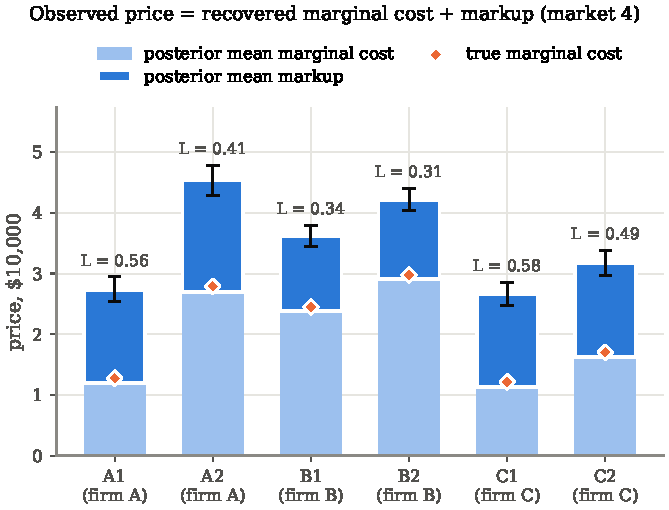
\includegraphics[width=0.85\linewidth]{chapters/blp/figures/fig_price_decomposition.pdf}
\caption{GBC posterior decomposition of observed prices into marginal cost and markup in market
4, with 90\% intervals on the markup and the true marginal costs (diamonds). The label above each
bar is the posterior mean Lerner index.}
\label{blp:fig:decomp}
\end{figure}

The GBC prior is uniform on a box: $\alpha\in[0.4,2]$, $\sigma_p\in[0,1]$,
$\sigma_x\in[0,1.5]$, $\beta_0\in[0.5,3.5]$, $\beta_1\in[0,2]$, $\beta_2\in[-0.5,1.5]$,
$\gamma_0\in[1,3]$, $\gamma_1\in[0,1]$, $\gamma_2\in[0,0.6]$, $\sigma_\xi\in[0.2,1]$,
$\sigma_\omega\in[0.1,0.6]$, $\rho\in[-0.5,0.5]$, with each conduct model equally likely. A draw is kept only if the solver converges with every price in $(0,60)$, in units of \$10{,}000, every share above $10^{-7}$ and an inside share below $0.995$ in every market (the local round below also requires the post merger equilibrium to solve). Failed draws are redrawn, parameters and shocks together, so the effective prior is the box density weighted by the probability that a draw of the shocks gives a valid equilibrium at those parameters, and the equal numbers per conduct make the three conduct models equally likely in the reference table. In that table 95 percent of the Bertrand Nash draws and 98 percent of the joint monopoly draws were kept, but only 50 percent of the perfect competition draws. Of the 2{,}948 rejected perfect competition draws, 2{,}776 had a price of zero or below and 172 an inside share of 0.995 or more; since prices equal costs under perfect competition, the effective prior for that conduct is concentrated on parameters that keep every cost positive. The other reference tables of the chapter kept 87 to 98 percent of their draws. The
amortized reference table has 3{,}000 industries per conduct model. A local second round draws
8{,}000 Bertrand Nash industries from the prior truncated to a box covering the first round
posterior and records the estimands; its posterior uses the 1{,}500 residuals nearest the fit at $S^{\mathrm{obs}}$, unweighted. We compare with logit IV, BLP GMM (two step, sandwich
standard errors, 250 Krinsky and Robb draws for derived quantities) and the Bayesian inversion MCMC of
Section~\ref{blp:sec:existing} (one chain of 5{,}000 iterations, the first 1{,}500 discarded). The seeded chain's path depends on numerical libraries: runs on other machines moved the posterior mean of $\alpha$ in its second decimal and its posterior standard deviation by less than 0.005. No comparison below turns on this Monte Carlo noise. The exogenous design $(\bm x,\bm w)$ is held fixed, so every procedure conditions on it.

Every true value and estimate in this chapter uses the 200 simulated consumers that generated the data. Holding the observed shares and prices fixed, using 3{,}200 antithetic normal draws instead moves the true merger price effect from 13.3 to 14.5 percent and the industry Lerner index from 0.434 to 0.454. The effect at the GMM estimate moves from 12.7 to 13.4 percent. These application shifts are smaller than the corresponding posterior standard deviations in Table~\ref{blp:tab:main}, but larger than its rounding. Across 50 Bertrand Nash industries drawn from the prior, the median change in the merger effect is 1.5 percentage points and the largest is 11.3. The reported results therefore describe the model with 200 consumers.

Numerical searches support the computed equilibria. The solver reaches the same prices from six starting points. Before the merger, we check all 24 firm and market pairs in the first eight markets using a 160 by 160 grid of markups from 0.01 to 40 and 60 random quasi Newton starts. No search finds a profitable deviation, and the second order condition holds at every pair, with 200, 800, 3{,}200 and 12{,}800 draws. After the merger, a separate quasi Newton search from six starts finds no profitable deviation in the 16 firm and market pairs, with 200 and 3{,}200 draws.

\subsection{Conduct, demand parameters and markups}

\paragraph{Conduct.} In the space of markup regression loadings (Figure~\ref{blp:fig:conduct}),
the three conduct models separate as Lemma~\ref{blp:lem:logit} predicts, and the observed data sit inside the Bertrand Nash cloud. The posterior probability of
Bertrand Nash is \numpbert, and on the \numncal\ held out simulated industries of Section~\ref{blp:sec:calibration} the classifier recovers the true
conduct with balanced accuracy \numconductacc. With the posterior this concentrated, the model averaging of Proposition~\ref{blp:prop:bma} changes little, here and in Section~\ref{blp:sec:misspec}, where what changes the answer is estimating conduct instead of maintaining Bertrand Nash.

\begin{figure}[htbp]
\centering
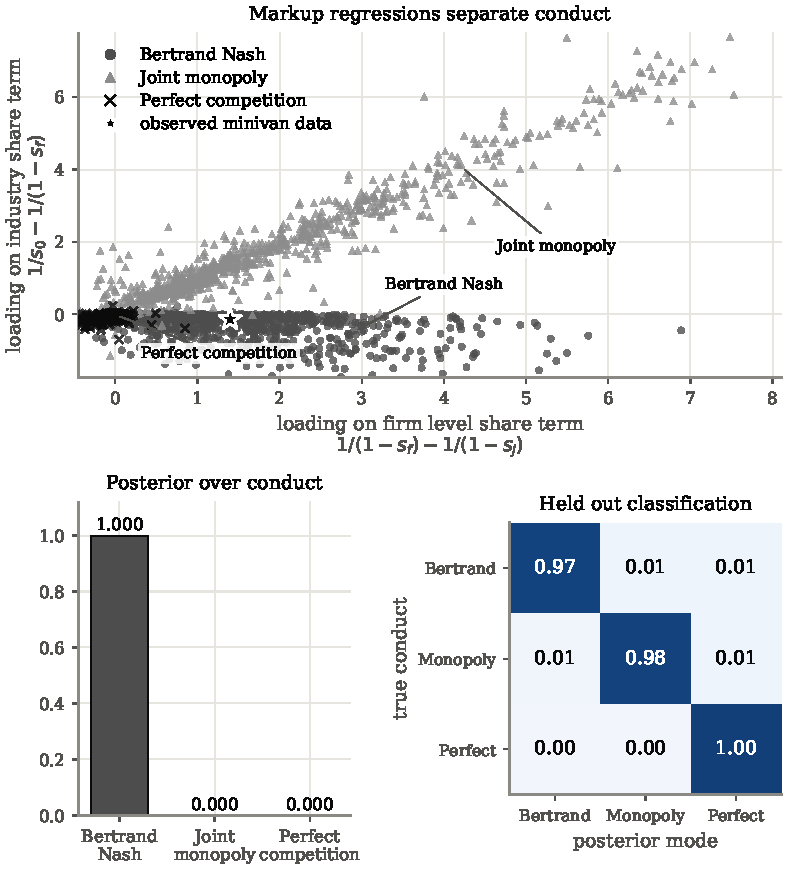
\includegraphics[width=\linewidth]{chapters/blp/figures/fig_conduct.pdf}
\caption{Top: loadings of prices on the nested markup regressors for simulated industries under
three conduct models; the star is the observed data. Bottom left: GBC posterior over conduct. Bottom right:
classification of conduct on held out simulated industries.}
\label{blp:fig:conduct}
\end{figure}

\paragraph{Demand parameters and markups.} Table~\ref{blp:tab:main} and Figure~\ref{blp:fig:theta} report the demand parameters. Logit IV fixes $\sigma_p=\sigma_x=0$, imposing independence of irrelevant alternatives\index{independence of irrelevant alternatives|textbf}; in this industry it understates price sensitivity and overstates markups. BLP GMM recovers the parameters, but its standard error for $\sigma_p$ is nearly two fifths of the estimate. The micro moments
pin $\sigma_p$ down: the GBC posterior standard deviation of $\sigma_p$ falls from
\numspnomicro\ without them to \numspmicro\ with them. The inversion MCMC, which conditions on the full data, has a posterior standard deviation for $\alpha$ of 0.050 against 0.087 for the local GBC posterior with micro moments. Part of that gap may be the price of conditioning on summaries, but the two posteriors also differ in likelihood (a reduced form for price against the equilibrium) and in prior, so the comparison does not isolate it. For $\sigma_p$ the order reverses (0.067 against 0.047) because the inversion MCMC does not use the micro moments. Figure~\ref{blp:fig:ridge} shows why markups
are about as well determined as $\alpha$ and better than $\sigma_p$: $\alpha$ and $\sigma_p$ trade off along a
ridge on which $\E[\alpha_i]$ is nearly constant, and the implied Lerner index tracks
$1/\E[\alpha_i]$ to a degree (correlation \numcorrLa). Figure~\ref{blp:fig:lerner} reports product level Lerner
indices.

\begin{table}[htbp]
\centering\footnotesize\setlength{\tabcolsep}{2.5pt}
\resizebox{\linewidth}{!}{\begin{tabular}{lcccccc}
\toprule
 & $\alpha$ & $\sigma_p$ & $\sigma_x$ & Lerner & $\Delta p/p$, \% & $\Delta$CS \\
\midrule
\csname @@input\endcsname chapters/blp/table_main.tex 
\bottomrule
\end{tabular}}
\caption{Posterior means (standard deviations) of the nonlinear demand parameters and of the
antitrust estimands obtained by plugging in parameter draws, for the Bayesian rows (GBC and the inversion MCMC). For GMM and logit the parameter columns give the point estimate and its sandwich standard error, and the derived quantities the mean (standard deviation) of Krinsky and Robb draws from the asymptotic normal approximation. $\Delta p/p$ is the
average over the four merging products; $\Delta$CS is per consumer per market in units of
\$10{,}000.}
\label{blp:tab:main}
\end{table}

\begin{figure}[htbp]
\centering
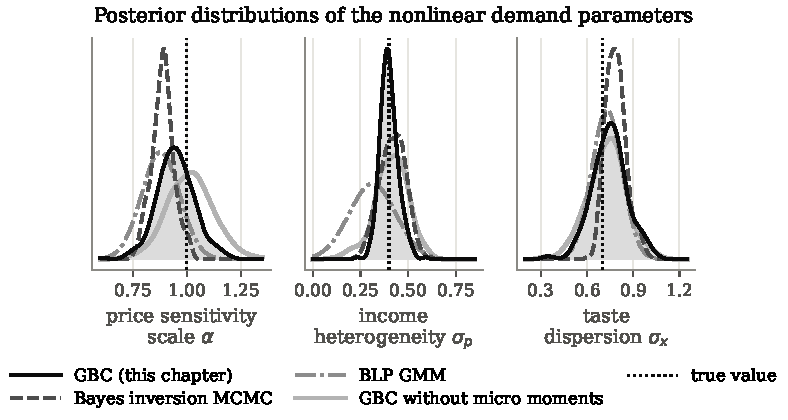
\includegraphics[width=\linewidth]{chapters/blp/figures/fig_theta_posteriors.pdf}
\caption{Posterior distributions of $\theta_2$. GMM is shown as its asymptotic normal
approximation.}
\label{blp:fig:theta}
\end{figure}

\begin{figure}[htbp]
\centering
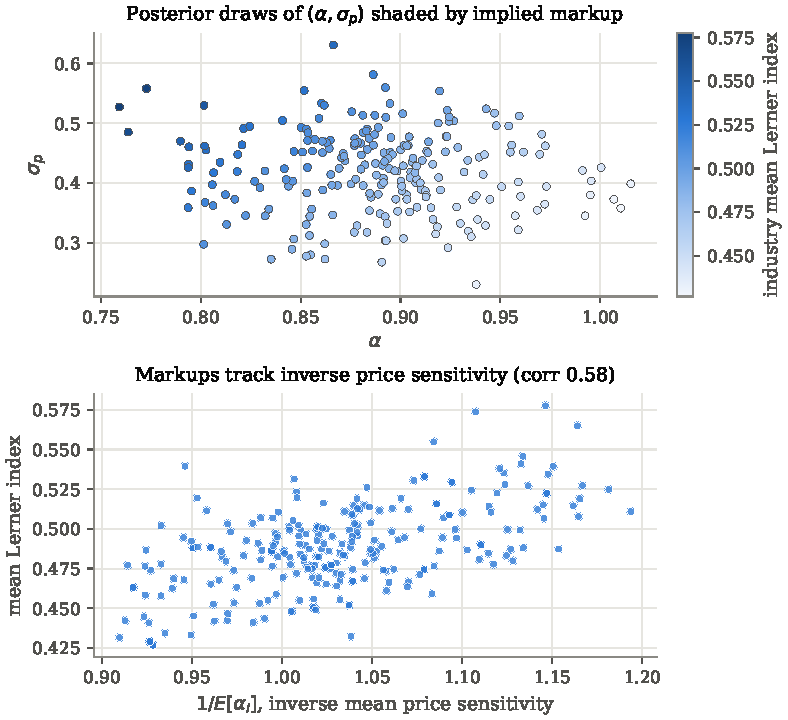
\includegraphics[width=\linewidth]{chapters/blp/figures/fig_markup_ridge.pdf}
\caption{Top: posterior draws of $(\alpha,\sigma_p)$ from the Bayesian inversion MCMC, shaded by
the industry mean Lerner index they imply. Bottom: the Lerner index against the inverse of mean
price sensitivity.}
\label{blp:fig:ridge}
\end{figure}

\begin{figure}[htbp]
\centering
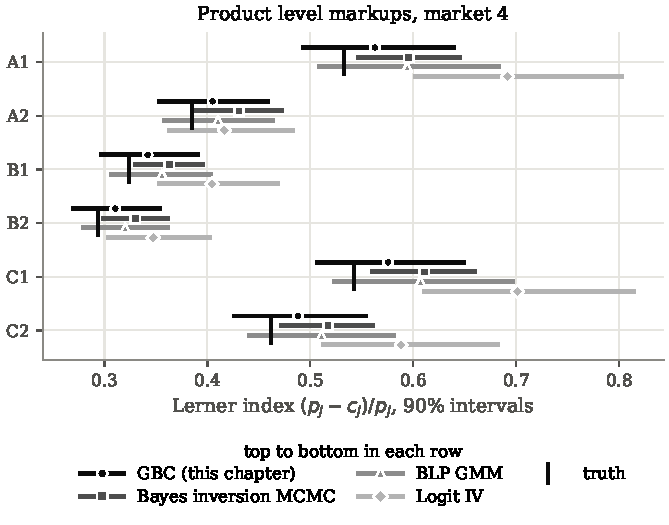
\includegraphics[width=0.85\linewidth]{chapters/blp/figures/fig_lerner_forest.pdf}
\caption{Product level Lerner indices in market 4, 90\% intervals by method, with the truth.}
\label{blp:fig:lerner}
\end{figure}

\subsection{Substitution, screens and the merger}
Figure~\ref{blp:fig:diversion} compares diversion ratios. The logit spreads diversion in proportion
to shares, $\mathrm{DR}_{jk} = s_k/(1-s_j)$, while the random coefficients posterior sends more diversion
to products with similar $x_1$, the pattern that matters when merging products are close in characteristic space. Figure~\ref{blp:fig:guppi} shows the posterior
GUPPI of each merging model; the probability of exceeding a 5\% screen is \numguppia\ for each of A1, A2, B1 and B2.

\begin{figure}[htbp]
\centering
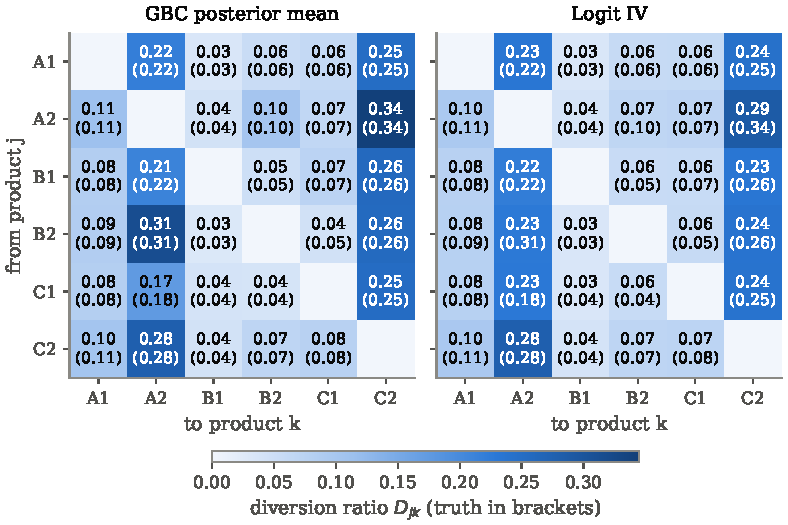
\includegraphics[width=\linewidth]{chapters/blp/figures/fig_diversion.pdf}
\caption{Diversion ratios in market 4: GBC posterior means and logit, with the truth in brackets.}
\label{blp:fig:diversion}
\end{figure}

\begin{figure}[htbp]
\centering
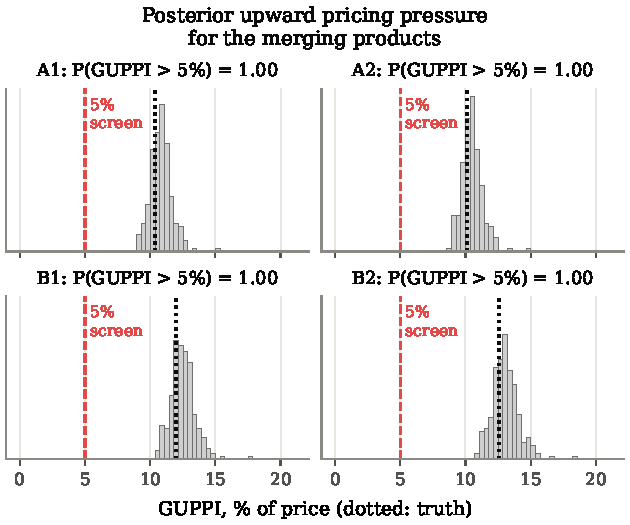
\includegraphics[width=0.8\linewidth]{chapters/blp/figures/fig_guppi.pdf}
\caption{Posterior GUPPI for the four merging products (market averages), with the truth
(dotted) and a 5\% screen.}
\label{blp:fig:guppi}
\end{figure}

Figure~\ref{blp:fig:merger} shows the merger simulation. In truth the prices of the merging models rise
by between 12\% and 15\% and those of the outsider C by 1.5\%, the strategic complement response;
the GBC posterior means are within about half a percentage point of each. Logit IV reports a merging
party price increase of \numdplogit\% against a true \numdptrue\%. The direct GBC estimand posterior (Figure~\ref{blp:fig:estimands}) gives a merging party price increase of $\numdpdir\%$
(s.d. \numdpdirsd), an industry Lerner index of $\numldir$ (s.d. \numldirsd) and a consumer
surplus change of $\numcsdir$ (s.d. \numcsdirsd), against true values of $\numdptrue\%$,
$\numltrue$ and $\numcstrue$.

\begin{figure}[htbp]
\centering
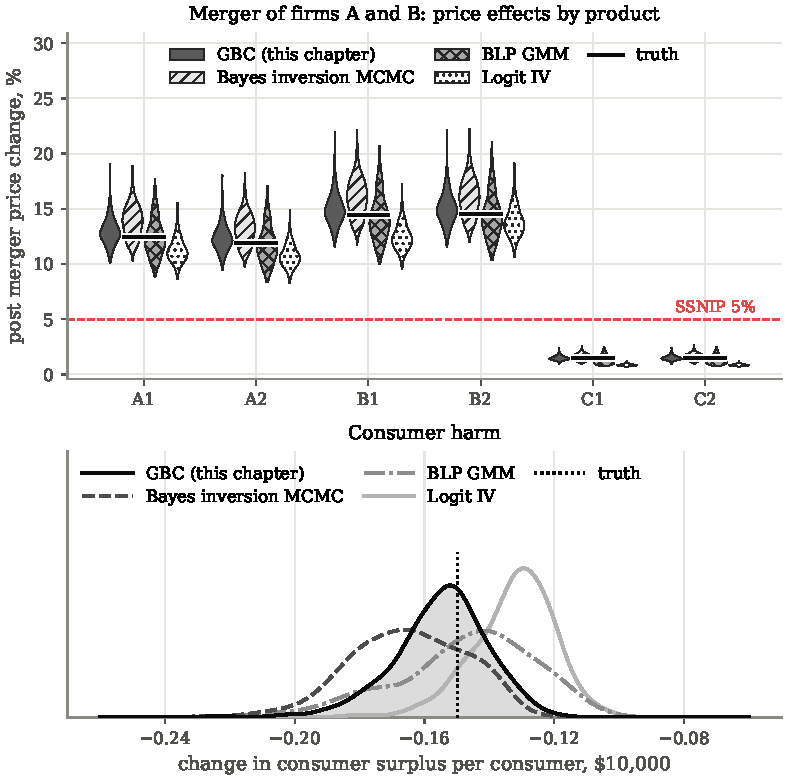
\includegraphics[width=\linewidth]{chapters/blp/figures/fig_merger.pdf}
\caption{Merger of manufacturers A and B. Top: price changes by product, averaged
over markets, from posterior draws (GBC, Bayes inversion MCMC) and Krinsky and Robb draws (BLP GMM, logit IV). Bottom: the same draws for the change in consumer surplus per consumer.}
\label{blp:fig:merger}
\end{figure}

\begin{figure}[htbp]
\centering
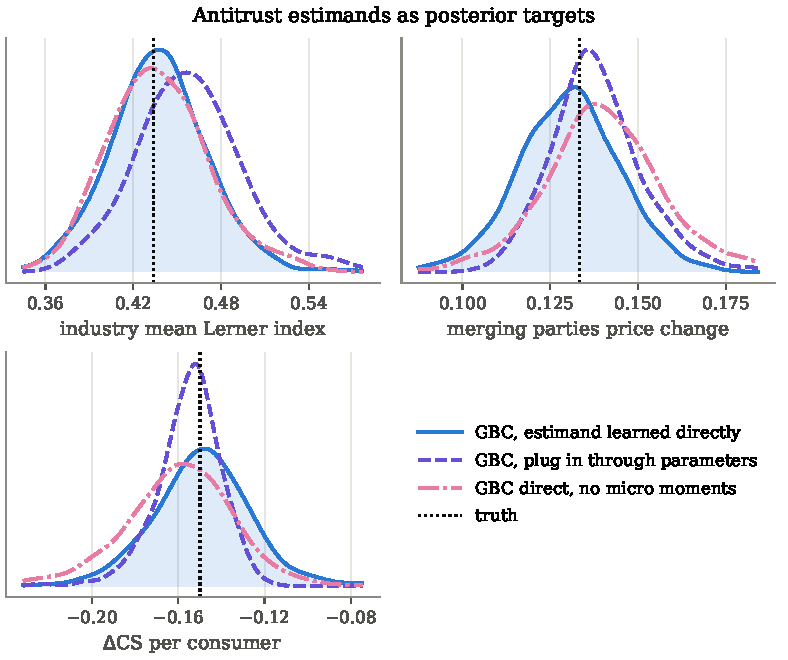
\includegraphics[width=\linewidth]{chapters/blp/figures/fig_estimands.pdf}
\caption{Antitrust estimands learned directly by GBC, compared with plugging GBC parameter draws
into Propositions \ref{blp:prop:markup} and \ref{blp:prop:merger}, and with the direct estimand learned
without micro moments.}
\label{blp:fig:estimands}
\end{figure}

\subsection{The decision}
Every method puts essentially all its mass, posterior or Krinsky and Robb, above the 5\% threshold and so reaches the same decision to challenge. Remedies and divestiture sizing, however, turn on the size of the effect. Figure~\ref{blp:fig:decision} plots $\Prob(\Delta p/p > r\mid\text{data})$ against $r$,
the input to Proposition~\ref{blp:prop:decision}. The GBC curve is the posterior of the estimand learned directly as a target, while the GBC rows of Table~\ref{blp:tab:main} plug in parameter draws. At $r = 12\%$ the GBC probability is
\numpgbcxii{} against \numplogitxii{} for logit IV; at $r=15\%$ it is \numpgbcxv{} against
\numplogitxv. By understating substitution between close products, logit understates the probability of large harm.

The curve in Figure~\ref{blp:fig:decision} is the whole output of the analysis as far as the decision is concerned. Read it at the harm threshold $r$ and compare its height with $\ell_1/(\ell_1+\ell_2)$, the cost of a wrongful challenge divided by the sum of the two error costs\index{merger!losses from wrongful challenge and clearance|textbf} (Proposition~\ref{blp:prop:decision}). A court that weighs the two errors equally compares it with $0.5$, an agency that regards underenforcement as nine times as costly with $0.1$, and both use the same curve. A confidence interval for $\Delta p/p$ supports none of this directly, because it fixes the error probability in advance and reports a set, whereas the agency wants to fix the set, the harmful region above $r$, and learn the probability.



\begin{figure}[htbp]
\centering
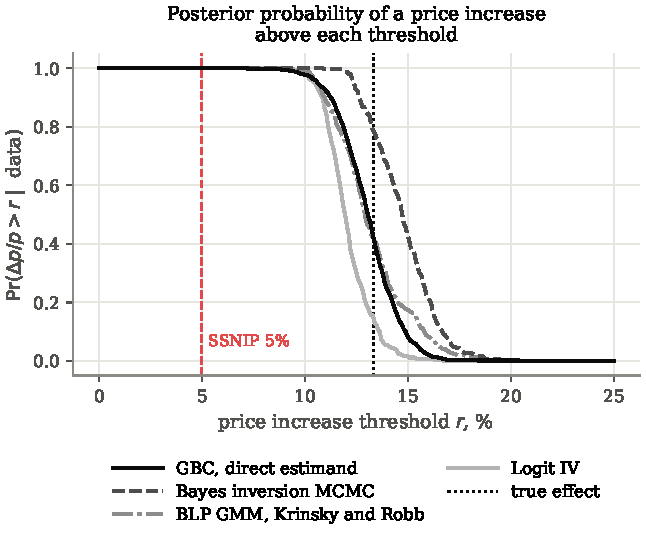
\includegraphics[width=0.82\linewidth]{chapters/blp/figures/fig_decision.pdf}
\caption{Probability that the merging parties' average price increase exceeds
$r$: the posterior for GBC and for the Bayesian inversion MCMC, and Krinsky and Robb draws for BLP GMM and logit IV. It is the input to the Bayes rule of Proposition~\ref{blp:prop:decision}.}
\label{blp:fig:decision}
\end{figure}

\section[A cereal merger and its remedy]{An antitrust case: a cereal merger with a divestiture remedy}\label{blp:sec:cereal}

Merger review rarely ends with a yes or no on the merger as proposed: the parties offer remedies\index{merger!remedy|textbf}, typically divestitures, and the agency must decide whether they restore competition. This case is patterned on ready to eat cereal\index{merger!cereal example with a divestiture|textbf} (Nevo 2000).

Eight brands are sold by four firms: a leader A with
three brands, B and C with two each, and a fringe firm D with one, observed in $T=30$ city markets.
Inside shares are \numcershA\% for A, \numcershB\% for B, \numcershC\% for C and \numcershD\% for D, so inside goods hold \numcerinside\% of the market. Demand and costs follow Section~\ref{blp:sec:model}, with the parameters of Section~\ref{blp:sec:app} except the demand intercept, $\beta_0 = 1.2$ rather than 2, and Bertrand Nash pricing.

Firms B and C, the second and third largest, propose to merge. The agency considers divesting C2 to the fringe firm D and asks whether it brings the price effect below 5\%.

GBC is trained once on 6{,}000 simulated Bertrand Nash industries at this
design, with five estimands as targets: the industry Lerner index, and the average price effect over the merging parties' four brands B1, B2, C1 and C2 (C2 included after it is divested) and the consumer surplus change per consumer, each with and without the remedy. Each is computed exactly in every simulated industry from the two post merger equilibria (Proposition~\ref{blp:prop:merger} with $H^{\mathrm{post}}$ set by the merger or by the
remedied ownership). Parameters are drawn from the prior of Section~\ref{blp:sec:app}, the two micro moments enter the summaries with their survey noise, and the posterior uses the 1{,}500 residuals nearest the fit at the observed summaries. BLP GMM is fitted to the same data, with estimands from plugging in $\hat\theta_2$ and 150 Krinsky and Robb draws for uncertainty.

\begin{table}[htbp]
\centering\small
\resizebox{\linewidth}{!}{\begin{tabular}{lcc}
\toprule
 & Merger & Merger with divestiture of C2 \\
\midrule
Truth & \numcerdpmtrue\% & \numcerdprtrue\% \\
GBC posterior mean (s.d.) & \numcerdpmgbc\% (\numcerdpmgbcsd) & \numcerdprgbc\% (\numcerdprgbcsd) \\
BLP GMM (Krinsky and Robb s.d.) & \numcerdpmgmm\% (\numcerdpmgmmsd) & \numcerdprgmm\% (\numcerdprgmmsd) \\
Logit IV & \numcerdpmlogit\% & \numcerdprlogit\% \\
\midrule
GBC $\Prob(\Delta p/p > 5\%\mid\data)$ & \numcerpmgbc & \numcerprgbc \\
GMM $\Prob(\Delta p/p > 5\%)$, Krinsky and Robb & \numcerpmgmm & \numcerprgmm \\
\midrule
True $\Delta$CS per consumer & $\numcercsmtrue$ & $\numcercsrtrue$ \\
GBC posterior mean $\Delta$CS & $\numcercsmgbc$ & $\numcercsrgbc$ \\
\bottomrule
\end{tabular}}
\caption{The cereal case: merging parties' average price effect and consumer surplus change, with
and without the remedy.}
\label{blp:tab:cereal}
\end{table}

\begin{figure}[htbp]
\centering
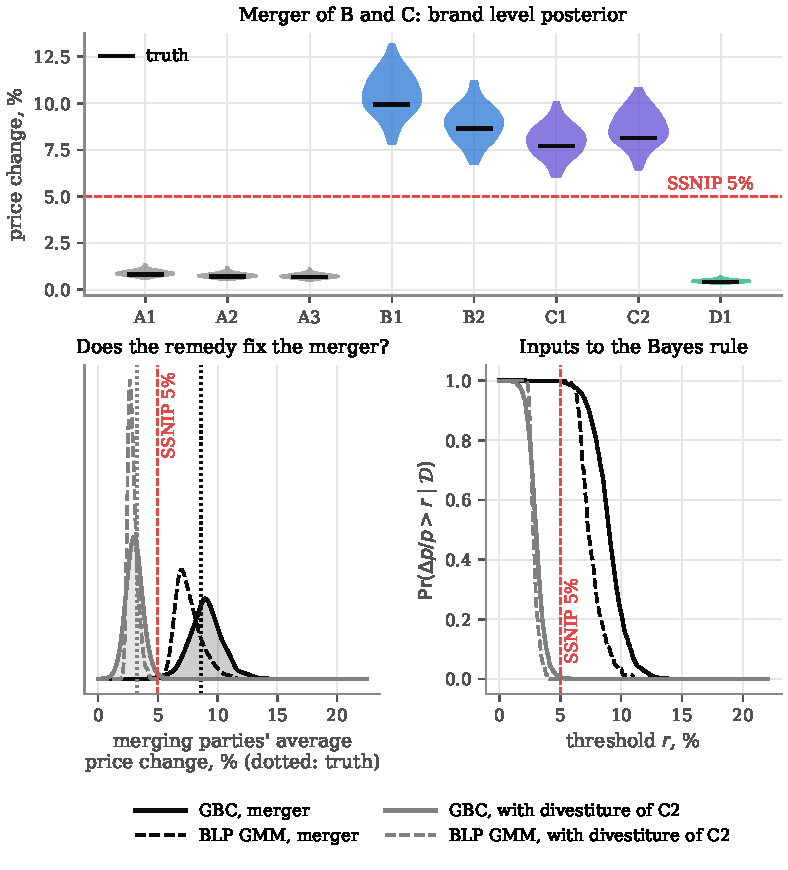
\includegraphics[width=\linewidth]{chapters/blp/figures/fig_cereal.pdf}
\caption{The cereal case. Top: GBC posterior of brand level price effects of the B and C merger.
Bottom left: posterior of the merging parties' average price effect with and without the divestiture,
GBC (solid) and BLP GMM (dashed); black is the merger as proposed and gray the remedy, here and in the bottom right panel. Bottom right: $\Prob(\Delta p/p>r\mid\data)$, the input to
Proposition~\ref{blp:prop:decision}.}
\label{blp:fig:cereal}
\end{figure}

Table~\ref{blp:tab:cereal} and Figure~\ref{blp:fig:cereal} report three findings.
\begin{enumerate}
\item The true average price effect on the merging brands is \numcerdpmtrue\%. GBC
reports \numcerdpmgbc\% with posterior standard deviation \numcerdpmgbcsd; BLP GMM reports
\numcerdpmgmm\% and logit \numcerdpmlogit\%. Both understate the effect in this industry. Logit fixes diversion in proportion to shares by independence of irrelevant alternatives\index{independence of irrelevant alternatives}, which need not match the substitution between the merging brands, so the sign of its error is a finding here and not a consequence of the model. B1 and B2 rise most because their partner C has the larger share (\numcershC\% against \numcershB\%), as Lemma~\ref{blp:lem:pressure} predicts under logit, where markup pressure on $f$ is increasing in $s_n$; with random coefficients the lemma is an approximation.
\item Divesting C2 removes about half the partner's share and, by
Lemma~\ref{blp:lem:pressure}, more than half of the markup pressure on B. The true effect falls to
\numcerdprtrue\%. GBC gives \numcerdprgbc\% (s.d. \numcerdprgbcsd) and BLP GMM \numcerdprgmm\% with a
Krinsky and Robb standard deviation of \numcerdprgmmsd. The posterior standard deviation is three times larger, but a few extreme draws inflate it (item 3), and the true remedied effect lies within 1.645 Krinsky and Robb standard deviations of the GMM estimate, so on this data set the narrower GMM band is not shown to be overconfident.
\item With equal error costs, $\ell_1 = \ell_2$, Proposition~\ref{blp:prop:decision} challenges
when $\Prob(\Delta p/p > 5\%\mid\data) > 0.5$. GBC gives \numcerpmgbc{} for the merger and
\numcerprgbc{} with the remedy, so the Bayes rule challenges the merger as proposed and accepts the
remedy. The entry for the remedy is a count of posterior draws, \numcerprgbcnabove{} of \numcerngbcdraws{} above 5 percent. A normal curve with the mean and standard deviation of the table would give 0.06, but a few extreme draws inflate that standard deviation: 90 percent of the draws lie between \numcerdprgbcqlo{} and \numcerdprgbcqhi{} percent. An agency weighing underenforcement more heavily, say $\ell_2 = 9\ell_1$, challenges whenever the probability exceeds $0.1$ and still accepts the remedy. The GMM probabilities lead to the same actions here, but with an understated merger effect; the consumer surplus loss the remedy avoids, $\numcercsrgbc - (\numcercsmgbc) = 0.039$ per
consumer under GBC, is what sizes the divestiture.
\end{enumerate}

\section[Repeated sampling]{Repeated sampling: GBC against BLP GMM}\label{blp:sec:mc}

One data set cannot separate method from luck, so we redraw the
unobservables $(\bm\xi,\bm\omega)$ and the micro survey noise \nummcnxv{} times with the design and
the true parameters fixed, at $T=40$ and at $T=15$ markets\index{simulation study!repeated sampling, GBC against BLP GMM|textbf}. In each
replication we fit BLP GMM\index{BLP GMM!against generative Bayesian computation|textbf} (three starting values, two step, sandwich covariance, 100 Krinsky and
Robb draws pushed through Propositions \ref{blp:prop:markup} and \ref{blp:prop:merger}; the GMM point
estimate of an estimand is the median of these draws, and Table~\ref{blp:tab:mcplug} adds the plug in $g(\hat\theta_2)$) and the amortized GBC posterior, trained once per design on 6{,}000 Bertrand
Nash industries drawn from the prior, and its posterior uses the 1{,}500 residuals nearest the fit at the summaries of the replication, unweighted. The amortized posterior is less sharp than the local second round on the data set of Section~\ref{blp:sec:app}, so this comparison is probably conservative for GBC, although we did not run the local round in repeated sampling.

Table~\ref{blp:tab:mc} and Figures \ref{blp:fig:mcerr} and \ref{blp:fig:mccov} report bias, root mean
squared error, coverage of nominal 90\% intervals and median interval length, and Table~\ref{blp:tab:mcse} their Monte Carlo standard errors. Six findings
follow.

\begin{enumerate}
\item The root mean squared error of the merger price effect, in percentage points, is \nummcdprmsegbcxl{} for GBC against \nummcdprmseplugxl{} for the GMM plug in $g(\hat\theta_2)$ at $T=40$, and \nummcdprmsegbcxv{} against \nummcdprmseplugxv{} at $T=15$ (Table~\ref{blp:tab:mcplug}). GBC has the larger absolute bias (Table~\ref{blp:tab:mc}, against \nummcdpbiasplugxl{} and \nummcdpbiasplugxv{} for the plug in) and the smaller variance. Taking the median of the Krinsky and Robb draws as the GMM estimate, as Table~\ref{blp:tab:mc} does, raises its error to \nummcdprmsegmmxl{} at $T=40$ and \nummcdprmsegmmxv{} at $T=15$, the latter with Monte Carlo standard error \nummcdprmsesegmmxv{} and driven by the replications of item 2 whose draws explode. GMM is nearly unbiased for $\alpha$; its weakness is the variance parameter and everything downstream. Root
mean squared error for $\sigma_p$ is \nummcsprmsegbcxl{} for GBC against \nummcsprmsegmmxl{} for
GMM at $T=40$, and \nummcsprmsegbcxv{} against \nummcsprmsegmmxv{} at $T=15$.
\item The GMM estimate of $\sigma_p$ is below $0.05$ in \nummcboundxv{} of
\nummcnxv{} replications at $T=15$ (\nummcboundxl{} at $T=40$). In \nummcexplxv{} replications at
$T=15$ the Krinsky and Robb distribution of the merger effect has its 95th percentile above
100\%, because a normal approximation near the boundary puts mass on large $\sigma_p$ and
hence on consumers with almost no price sensitivity. 
\item GBC intervals are conservative, covering at 0.95 to 1.00, while
GMM intervals for the Lerner index cover at \nummclercovgmmxl{} at $T=40$ and \nummclercovgmmxv{} at $T=15$, with Monte Carlo standard errors \nummclercovsegmmxl{} and \nummclercovsegmmxv{}. That is 2.5 and 7 Monte Carlo standard errors below 0.90, so the undercoverage is clear at $T=15$ and likely at $T=40$. GBC intervals for $\sigma_p$ are about half
as long as GMM's (\nummcsplengbcxl{} against \nummcsplengmmxl{} at $T=40$); for the merger effect
the lengths are similar.
\item Part of the GBC advantage comes from the micro moments, which aggregate BLP does not use; removing them raises its root mean squared error for $\sigma_p$ to
\nummcsprmsenmxl{} ($T=40$) and \nummcsprmsenmxv{} ($T=15$), and for the merger effect to
\nummcdprmsenmxl{} and \nummcdprmsenmxv{}, still below GMM in every case, although at $T=40$ the gap for $\sigma_p$ is about three Monte Carlo standard errors and the GMM plug in for the merger effect (\nummcdprmseplugxl{}) comes close.
\item With $T=15$ the amortized GBC posterior for the industry Lerner index
is pulled towards the prior (bias 0.12), with wide intervals. The network was trained over the whole prior; the local second round of Section~\ref{blp:sec:app} should reduce this, at the cost of a second simulation round per data set, but we ran it only on the $T=40$ application.
\item With a true $\sigma_p$ of 0.05, near the boundary, and the rest of the design unchanged (\nummcfivexln{} replications at $T=40$, \nummcfivexvn{} usable at $T=15$), the GMM estimate of $\sigma_p$ is below $0.05$ in \nummcfivexlbound{} and \nummcfivexvbound{} of them, and its Wald intervals for $\sigma_p$ cover at \nummcfivespcovgmmxl{} and \nummcfivespcovgmmxv{}. The Krinsky and Robb intervals for the merger price effect cover at only \nummcfivedpcovgmmxl{} and \nummcfivedpcovgmmxv{}, and the median of the draws has root mean squared error \nummcfivedprmsegmmxl{} and \nummcfivedprmsegmmxv{} percentage points, against \nummcfivedprmsegbcxl{} and \nummcfivedprmsegbcxv{} for GBC, whose intervals cover at \nummcfivedpcovgbcxl{} and \nummcfivedpcovgbcxv{}. We did not compute the plug in for this design.
\end{enumerate}


\begin{table}[htbp]
\centering\footnotesize\setlength{\tabcolsep}{5pt}
\begin{tabular}{lcccccccc}
\toprule
 & \multicolumn{4}{c}{BLP GMM} & \multicolumn{4}{c}{GBC} \\
\cmidrule(lr){2-5}\cmidrule(lr){6-9}
 & bias & RMSE & cover & length & bias & RMSE & cover & length \\
\midrule
\csname @@input\endcsname chapters/blp/table_mc.tex 
\bottomrule
\end{tabular}
\caption{Repeated sampling performance. Coverage and length refer to nominal 90\% intervals:
Wald for GMM parameters, Krinsky and Robb for GMM estimands, posterior quantiles for GBC. The
truth of the estimands varies across replications with $(\bm\xi,\bm\omega)$ and is computed
exactly in each.}
\label{blp:tab:mc}
\end{table}

\begin{figure}[htbp]
\centering
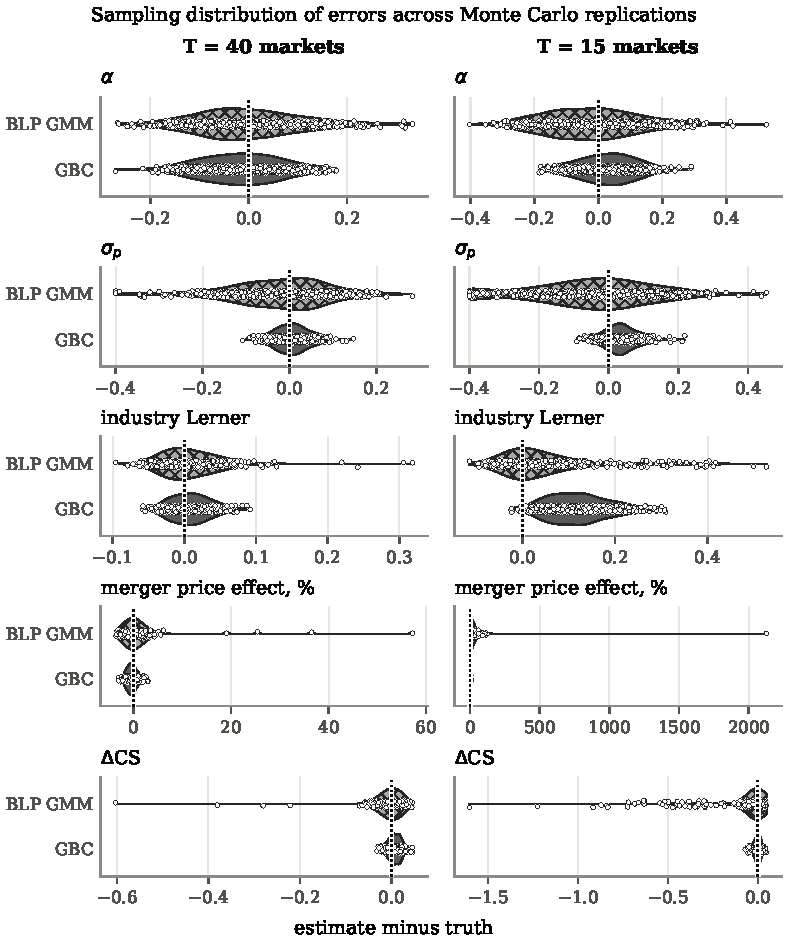
\includegraphics[width=\linewidth]{chapters/blp/figures/fig_mc_errors.pdf}
\caption{Errors across Monte Carlo replications, BLP GMM point estimates against GBC posterior
means, with $T=40$ (left) and $T=15$ (right) markets.}
\label{blp:fig:mcerr}
\end{figure}

\begin{figure}[htbp]
\centering
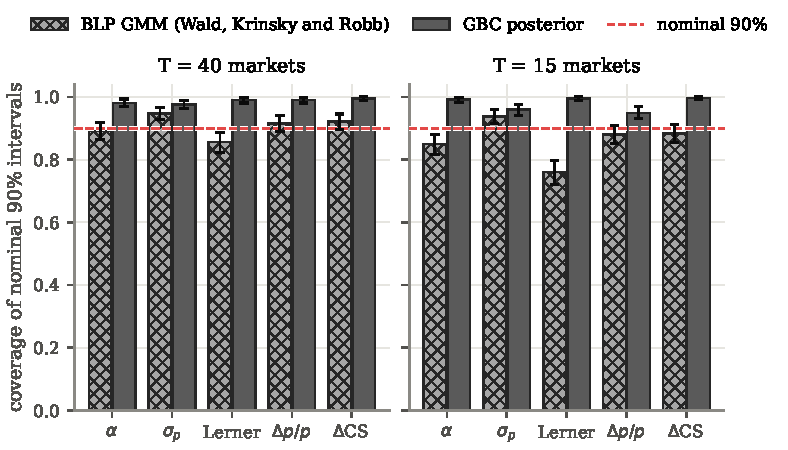
\includegraphics[width=\linewidth]{chapters/blp/figures/fig_mc_coverage.pdf}
\caption{Coverage of nominal 90\% intervals across Monte Carlo replications.}
\label{blp:fig:mccov}
\end{figure}

\begin{table}[htbp]
\centering\footnotesize\setlength{\tabcolsep}{5pt}
\begin{tabular}{lcccc}
\toprule
 & \multicolumn{2}{c}{Median of Krinsky and Robb draws} & \multicolumn{2}{c}{Plug in $g(\hat\theta_2)$} \\
\cmidrule(lr){2-3}\cmidrule(lr){4-5}
 & bias & RMSE & bias & RMSE \\
\midrule
\csname @@input\endcsname chapters/blp/table_mc_plug.tex 
\bottomrule
\end{tabular}
\caption{Two GMM point estimates of the estimands in the design of Table~\ref{blp:tab:mc} (true $\sigma_p=0.4$, 500 replications at each $T$): the median of the 100 Krinsky and Robb draws, as in that table, and the plug in of the GMM estimate $\hat\theta_2$.}
\label{blp:tab:mcplug}
\end{table}

\begin{table}[htbp]
\centering\footnotesize\setlength{\tabcolsep}{5pt}
\begin{tabular}{lcccccccc}
\toprule
 & \multicolumn{4}{c}{BLP GMM} & \multicolumn{4}{c}{GBC} \\
\cmidrule(lr){2-5}\cmidrule(lr){6-9}
 & bias & RMSE & cover & length & bias & RMSE & cover & length \\
\midrule
\csname @@input\endcsname chapters/blp/table_mc_se.tex 
\bottomrule
\end{tabular}
\caption{Monte Carlo standard errors of the entries of Table~\ref{blp:tab:mc}, from 500 replications: for a bias, the standard deviation of the error over $\sqrt{500}$; for a root mean squared error, the standard deviation of the squared error over twice the root mean squared error times $\sqrt{500}$; for a coverage $c$, $\sqrt{c(1-c)/500}$. Interval lengths are medians and carry no standard error here.}
\label{blp:tab:mcse}
\end{table}

\section{Calibration on fresh industries}\label{blp:sec:calibration}

Intervals used in litigation should mean what they say across the industries a procedure might face, not only at one true parameter. Because the GBC posterior is amortized, we check this on \numncal\ fresh industries\index{calibration!on fresh industries|textbf} drawn from the prior under all three conduct models (the draws, of 450, that produced a valid equilibrium), each needing one simulation and one network evaluation; the intervals are those of the posterior given the true conduct, so conduct uncertainty is not part of this check. Figure~\ref{blp:fig:calibration}
reports coverage of nominal 90\% intervals for all twelve parameters. With in sample residuals the
average coverage is \numcovnaive; with cross fitted residuals it is \numcovavg, slightly conservative and never below
\numcovmin, and the probability integral transforms are roughly flat, with too little mass in the outer bins for $\alpha$, as slightly conservative intervals imply. The cross fitted intervals are slightly too wide because an out of fold residual carries the error of its fold network on top of the noise, while the prediction at $S^{\mathrm{obs}}$ averages the three fold networks and so carries less of that error.



The probabilities a hearing turns on can be checked the same way. On the \numncal\ fresh industries, the conduct classifier has Brier score 0.031, against 0.667 for equal probabilities. This score is the squared distance between the vector of conduct probabilities and the indicator vector for the true conduct, averaged over industries. The most probable conduct is correct in 98 percent of industries. Pooling the three probabilities per industry gives 1{,}062 values; only 17 lie between 0.1 and 0.9, too few to assess calibration in that range.

For the merger, whose effect the calibration industries do not record, we held out 1{,}000 industries of each Bertrand Nash reference table of Section~\ref{blp:sec:mc} ($T=40$ and $T=15$) and trained on the other 5{,}000. Table~\ref{blp:tab:calprob} compares posterior and base rate Brier scores and reports the calibration gap. The posterior's Brier score is 3 to 6 times smaller than the base rate's, and no gap exceeds 0.025. This check holds conduct fixed at Bertrand Nash.

\begin{table}[htbp]
\centering\footnotesize\setlength{\tabcolsep}{5pt}
\begin{tabular}{ccccc}
\toprule
$T$ & threshold $r$ (\%) & Brier, GBC & Brier, base rate & calibration gap \\
\midrule
40 & 5  & 0.016 & 0.062 & 0.009 \\
   & 12 & 0.042 & 0.220 & 0.019 \\
   & 15 & 0.039 & 0.249 & 0.013 \\
\midrule
15 & 5  & 0.025 & 0.083 & 0.015 \\
   & 12 & 0.060 & 0.244 & 0.025 \\
   & 15 & 0.063 & 0.245 & 0.019 \\
\bottomrule
\end{tabular}
\caption{Calibration of the GBC posterior probability that the merging parties' price effect exceeds $r$, on 1{,}000 held out Bertrand Nash industries at each $T$, with the network trained on the other 5{,}000. The Brier score is the mean squared difference between the predicted probability and the event indicator; the base rate predicts the observed frequency in the held out industries. The calibration gap is the mean absolute difference between predicted and observed frequencies over ten groups of 100 industries ordered by predicted probability.}
\label{blp:tab:calprob}
\end{table}

Calibration\index{calibration} over the prior does not guarantee calibration at any particular true parameter: at one such parameter, the Monte Carlo at $T=15$ shows the amortized Lerner posterior pulled towards the prior. And fresh industries come from the same demand and cost model that generated the training table, so this is a check on the computation, not on the economics; Section~\ref{blp:sec:misspec} checks the economics, as far as conduct goes.

\begin{figure}[htbp]
\centering
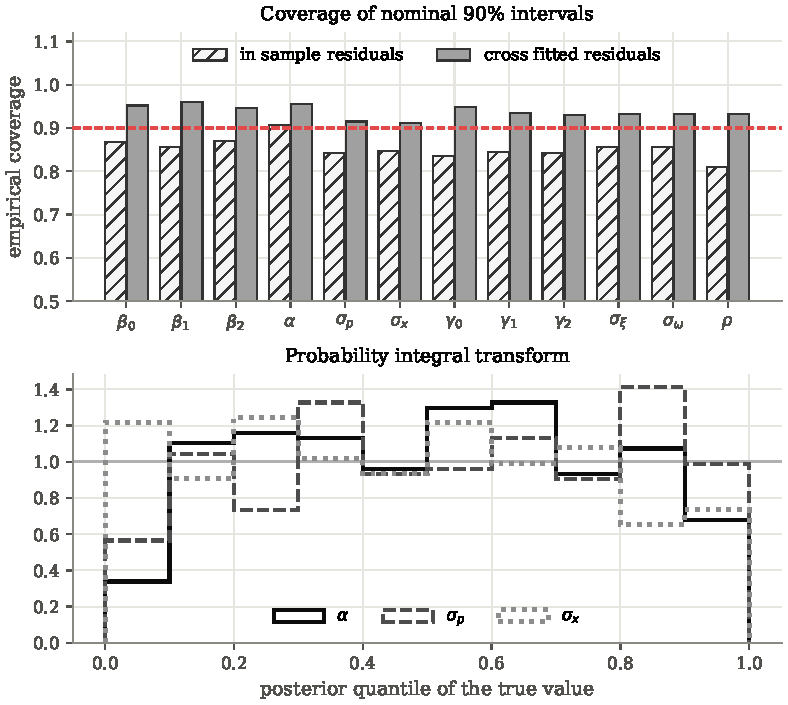
\includegraphics[width=\linewidth]{chapters/blp/figures/fig_calibration.pdf}
\caption{Calibration of GBC on held out industries, with the posterior given the true conduct. Top: coverage of nominal 90\% intervals with
in sample and with cross fitted residuals. Bottom: probability integral transform of the true
$\alpha$, $\sigma_p$ and $\sigma_x$ under the cross fitted posterior.}
\label{blp:fig:calibration}
\end{figure}

\section{When conduct is wrong}\label{blp:sec:misspec}

The experiment that matters most for policy generates one data set from the design of Section~\ref{blp:sec:app} under joint monopoly, and another under perfect competition, and asks each method to evaluate the A and B merger\index{conduct!wrong, misspecified|textbf}. BLP GMM, as is standard, estimates demand, then recovers costs and simulates the merger under Bertrand Nash at its point estimate, without Krinsky and Robb draws; GBC estimates conduct and uses 150 posterior draws.

\begin{itemize}
\item Collusive data\index{collusion|textbf}. A merger of two firms that already maximize joint profit changes nothing,
so the true price effect is \nummscollusiontrue\%. BLP GMM estimates demand well ($\hat\alpha = \nummscollusionalpha$) but, with Bertrand
supply, predicts \nummscollusiongmm\%, and recovers an industry Lerner index of \nummscollusionlgmm{} against a true
\nummscollusionltrue. GBC assigns posterior probability \nummscollusionpc{} to joint monopoly,
predicts \nummscollusiongbc\% and a Lerner index of \nummscollusionlgbc.
\item Competitive data. Prices equal costs and the true merger effect is \nummsperfecttrue\%.
BLP GMM again estimates demand well ($\hat\alpha = \nummsperfectalpha$) but Bertrand supply invents markups (Lerner \nummsperfectlgmm{} against
\nummsperfectltrue) and predicts \nummsperfectgmm\%. GBC assigns posterior probability
\nummsperfectpc{} to perfect competition and predicts \nummsperfectgbc\%.
\end{itemize}

Figure~\ref{blp:fig:misspec} summarizes. GMM's demand estimates are fine in both cases; the error comes entirely from the maintained supply side, which by Proposition~\ref{blp:prop:markup} determines costs and hence the counterfactual.

Estimating conduct helps only when the true conduct is among those in the reference table. In \nummspartn{} industries generated with the design of Section~\ref{blp:sec:app} and $T=40$ under partial internalization, each firm maximizing its own profit plus half of each rival's, a conduct outside the training set, the true merger price effect averages \nummsparttruedp\%. GBC puts on average probability \nummspartpcbert{} on Bertrand Nash and \nummspartpccoll{} on joint monopoly, and overstates the effect by \nummspartgbcbiasdp{} percentage points, about as much as BLP GMM with Bertrand Nash maintained (\nummspartgmmbiasdp{}; Monte Carlo standard errors \nummspartgbcsedp{} and \nummspartgmmsedp{}). Its posterior gives no sign that conduct is wrong.

\begin{figure}[htbp]
\centering
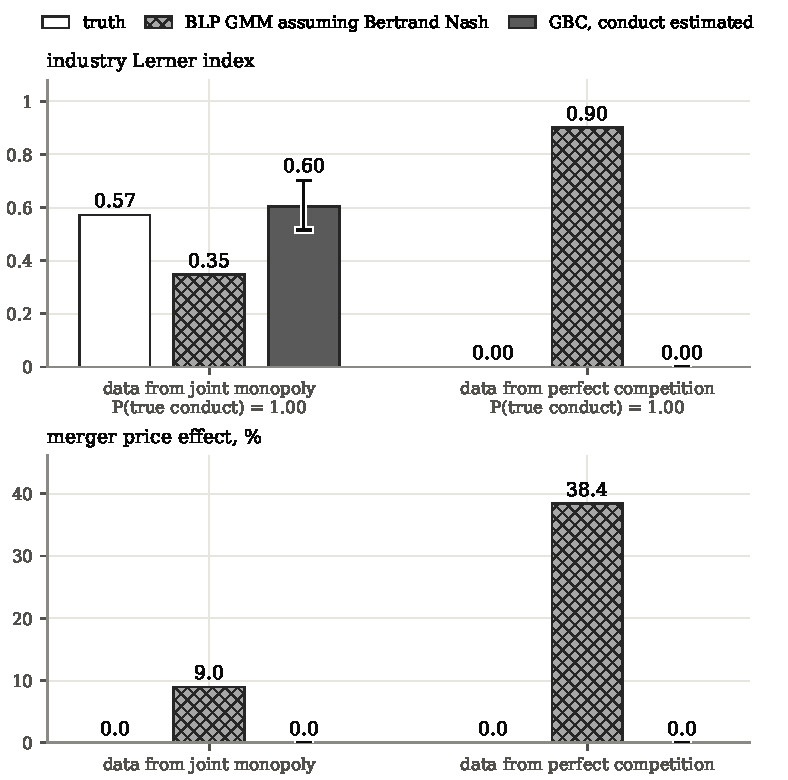
\includegraphics[width=\linewidth]{chapters/blp/figures/fig_misspec.pdf}
\caption{Merger evaluation when the data are generated by joint monopoly or by perfect
competition. BLP GMM maintains Bertrand Nash; GBC estimates conduct. Bars show the industry
Lerner index and the merging parties' price effect, with GBC 90\% intervals.}
\label{blp:fig:misspec}
\end{figure}

\section{Discussion}



The uncertainty that matters most is often structural: in Section~\ref{blp:sec:misspec} wrong conduct costs far more than sampling error in demand, and maintaining one conduct leaves this uncertainty out. A posterior over conduct is conditional on its candidate set. Duarte and coauthors (2024) give an example in which separate instrument sets favour different incorrect models, which reveals the misspecification without identifying the omitted true conduct.

Continuous conduct, such as conjectural variations or common ownership\index{common ownership|textbf} weights $H_{jk} = \kappa$ for rival products (Backus, Conlon and Sinkinson 2021), is one more coordinate of $\theta$ in Algorithm~\ref{blp:alg:gbc} (Exercise~\ref{blp:ex:kappa}). Merger efficiencies become a prior on the post merger change in $\bm c_t$, a controlled relaxation of modularity. Retrospective studies of past mergers can update the posterior for conduct and efficiencies.

\medskip\noindent\textit{Code.}\enspace The merger code and saved reference outputs are in \texttt{blp\_merger} (Appendix~\ref{app:code}).

\section{In practice}

\paragraph{The target.} The merger effect $\Delta\bm p_t$ is the intervention $\mathrm{do}(H := H^{\mathrm{post}})$ pushed through the equilibrium, and under modularity it is a function of $(\theta_2,H)$ and the data alone (Proposition~\ref{blp:prop:ident}). The decision input $\Prob(\Delta p/p > r\mid\data)$ is the fraction of posterior draws above $r$.

\paragraph{What the analyst does differently.} State the conduct models before estimating demand and report $\Prob(H\mid\data)$ rather than maintaining Bertrand Nash; in the collusive data the posterior of \nummscollusionpc{} on joint monopoly saves the decision. Fit the estimands as targets, so the merger effect is never a plug in through $\hat\theta_2$ (Proposition~\ref{blp:prop:pushforward}). Check calibration before use with cross fitted residuals (Section~\ref{blp:sec:calibration}). Report the curve $\Prob(\Delta p/p > r\mid\data)$ against $r$ rather than a point estimate with an interval, since the agency's loss ratio sets where it is read (Proposition~\ref{blp:prop:decision}). When markets are few, consider a local second round: the amortized posterior is pulled towards the prior at $T=15$, although we ran the second round only at $T=40$.

\paragraph{Against DML.} BLP GMM is already an orthogonal moment estimator: $\beta$ is profiled out and the concentrated criterion is insensitive to it at first order (Section~\ref{blp:sec:dml}, Exercise~\ref{blp:ex:dml}). A DML style treatment with cross fitted nuisances and an orthogonal score for $\theta_2$ inherits the same four limits: a fixed point target whose curvature bias orthogonality does not remove, moments flat in the random coefficient scales at zero (Proposition~\ref{blp:prop:flat}), a discrete conduct nuisance no score averages over, and an interval where a probability is needed. The evidence for BLP GMM is Section~\ref{blp:sec:mc}: root mean squared error for the merger effect in percentage points, GBC on the same aggregate data against GMM, of \nummcdprmsenmxl{} against \nummcdprmsegmmxl{} at $T=40$ (a gap of about 2.4 Monte Carlo standard errors) and \nummcdprmsenmxv{} against \nummcdprmsegmmxv{} at $T=15$, where Krinsky and Robb draws explode (\nummcdprmseplugxl{} and \nummcdprmseplugxv{} for the GMM plug in, which avoids the explosion); and the collusive data, where maintained Bertrand predicts \nummscollusiongmm\% for a true effect of \nummscollusiontrue\%. GMM is adequate with many markets, strong instruments, interior parameters and known conduct, where the two agree to first order and one optimization is cheaper than a reference table of thousands of industries.

\section{Notes and further reading}

Conlon and Gortmaker (2020) describe current BLP practice.
Merger simulation with differentiated products dates to Hausman, Leonard and Zona (1994) and
Werden and Froeb (1994), with Nevo (2000) an influential application; upward pricing
pressure is due to Farrell and Shapiro (2010); Miller and Weinberg (2017) combine conduct and
merger analysis in a modern case. Weinberg (2008) surveys retrospectives; Ashenfelter and Hosken (2010) is an example.

On the Bayesian side, Jiang, Manchanda and Rossi (2009) introduced the inversion likelihood, our benchmark, and
Gron, Polson and Viard (2003) and Viard, Gron and Polson (2015) the full equilibrium likelihood, with
equilibrium computation in Viard, Polson and Gron (2001). Generative Bayesian computation for causal problems is developed in
Nareklishvili, Polson and Sokolov (2023a); its regression adjustment ancestor is Beaumont, Zhang and Balding (2002), and the
asymptotics of summary based posteriors are in Frazier and coauthors (2018). The noise outsourcing lemma
is in Kallenberg (2002). 

\begin{exercises}
\item\label{ex:chapter_blp:1}\label{blp:ex:logit} Verify Lemma~\ref{blp:lem:logit} for a firm with products of different prices by solving the first order conditions, then show that under joint monopoly all markups equal $1/(\alpha s_0)$, and explain why the markup of a product does not depend on its own price, once shares are given, under multiproduct logit pricing.

\item\label{ex:chapter_blp:2}\label{blp:ex:outside} Suppose there is no outside good, so $s_{i0}=0$ for every consumer.
Show that the rows of $D_p^\top$ sum to zero, that $H^M\odot D_p^\top$ is singular, and hence that
joint monopoly markups are not defined. Interpret the result economically, and explain which step
of the proof of Lemma~\ref{blp:lem:dd} fails.

\item\label{ex:chapter_blp:3}\label{blp:ex:guppi} In Lemma~\ref{blp:lem:pressure} take $s_j = 0.10$, $s_f = 0.20$ and
$s_n = 0.15$, with $\alpha = 1$ and $p_j = 3$. Compute $\mathrm{GUPPI}_j$ and $\Delta m_j/p_j$.
By how much does GUPPI understate markup pressure? How does the ratio behave as $s_n$ grows?

\item\label{ex:chapter_blp:4}\label{blp:ex:flat} Extend Proposition~\ref{blp:prop:flat} to the income coefficient
$\alpha_i = \alpha e^{-\sigma_p\nu_i}$. Show that $\partial s_j/\partial\sigma_p = 0$ at
$\sigma_p = 0$ when $\E\nu_i = 0$, and compute the extra second order term that comes from
$\partial^2 e^{-\sigma\nu}/\partial\sigma^2 = \nu^2 e^{-\sigma\nu}$. Why do the micro moments
$\mu^{\mathrm{mic}}_1,\mu^{\mathrm{mic}}_2$ of Section~\ref{blp:sec:gbc} depend on $\sigma_p$ at first order?

\item\label{ex:chapter_blp:5}\label{blp:ex:bayesrule} In Proposition~\ref{blp:prop:decision}, suppose the agency regards
clearing a harmful merger as 49 times as costly as challenging a benign one. Find the
challenge threshold for $\Prob(\Delta p/p > r\mid\data)$. Using Table~\ref{blp:tab:cereal}, decide the
merger and the remedy under this loss.

\item\label{ex:chapter_blp:6}\label{blp:ex:bma} Suppose $\Prob(H^B\mid\data) = 0.7$ and $\Prob(H^M\mid\data) = 0.3$, with
conditional posterior means of the merger effect of 10\% and 0\%, and conditional standard
deviations of 1.5 and 0.5 percentage points. Use Proposition~\ref{blp:prop:bma} to compute the
posterior mean and standard deviation. What is the expected squared error of a procedure that
maintains Bertrand Nash?

\item\label{ex:chapter_blp:7}\label{blp:ex:interference} Using the potential outcome notation of
Section~\ref{blp:sec:causal}, define the effect of the A and B merger on the price of the
outsider's product C1. Explain why this effect is nonzero although C1's ownership does not change,
and use Proposition~\ref{blp:prop:firstorder} to show that to first order it equals the C1 row of
$(I-\nabla\bm m^{\mathrm{post}})^{-1}\Delta\bm m$, with $\Delta m_{C1} = 0$.

\item\label{ex:chapter_blp:8}\label{blp:ex:retro} A retrospective difference in differences study of an approved merger
reports a merging party price effect of 4\% with standard error 2\%, while the structural
posterior predicted 9\% with standard deviation 1.5\%. Treating the retrospective estimate as a
noisy observation of the realized effect, compute the posterior predictive probability, two sided, of a retrospective estimate at least as far from 9\% as 4\% is. Which parts of the model (demand, conduct, modularity) would you question
first, and how would you build them into the prior for the next case?

\item\label{ex:chapter_blp:9}\label{blp:ex:kappa} Common ownership. Replace $H$ by $H_{jk}(\kappa) = 1$ for $j,k$ with the
same owner and $\kappa\in[0,1]$ otherwise. Show that $\kappa = 0$ and $\kappa = 1$ recover
Bertrand Nash and joint monopoly. Modify \texttt{blp\_core.py} and the GBC targets to learn
$\kappa$, and report its posterior on the minivan data.

\item\label{ex:chapter_blp:10}\label{blp:ex:dml} Write BLP GMM with weighting matrix $\mathcal W$ as an estimating equation for $\theta_2$ with $\beta$ concentrated out. Verify that the $\beta$ gradient of the GMM criterion is zero at the profiled value and that the concentrated moment has zero derivative with respect to $\beta$. Then explain, using Proposition~\ref{blp:prop:pushforward}, why this orthogonality does not make $g(\hat\theta_2)$ unbiased for the merger effect.
\end{exercises}
